
\chapter[Typology of attribution marking]{A typology of adjective attribution marking devices} \label{ontology}
%%%
In the present chapter, different types of adjective attribution marking devices attested in natural languages will be described and systematized with a special focus on their typologization according to the morphology of attributive adjectives.

\section{Typologizing noun phrase structure}
%%%
The goal of the following chapters is to typologize noun phrases and to present a comprehensive ontology of different syntactic, morphosyntactic, and morpho-semantico-syntactic attribution marking devices attested in the languages spoken in northern Eurasia and beyond. 

In order to illustrate the different noun phrase types to which these devices belong, data from several languages both within and outside the geographic area of investigation are taken into consideration. The focus, however, will be on constructions and features especially relevant to adjective attribution in the northern Eurasian area.

The term \emph{adjective attribution marking} will be used to refer to a grammatical operation relating an adjectival modifier to its noun head. \emph{Attribution marking device} will be used to subsume both overt and covert grammatical operations which license the syntactic relation of attribution. 

The term \emph{noun phrase type} used here denotes the specific syntactic or morphosyntactic structure type of a noun phrase. This term is thus superordinate and belongs to noun phrase structure in general. Since the present study is restricted to a rather small subset of noun phrases, namely noun phrases with adjectival modifiers, the subordinated term \emph{adjective attribution marking device} (instead of \emph{adjective attribution marking type}) will be used to cover all grammatical operations which license the syntactic relation of adjective attribution.

\paragraph*{Attribution marking} Minimally, an attribution marking device will simply license the syntactic structure without licensing any of the constituents as head or dependent, i.e. without ranking single constituents. This is the case for the pure syntactic devices \emph{\isi{juxtaposition}} and \emph{\isi{incorporation}}.

The syntactic relation of attribution can also be licensed by a device linking the modifying and the modified constituents morphologically to each other, namely in the case of agreement marking. The morphological device of \emph{agreement marking}\is{agreement marking} is characterized by the assignment of an inherent (i.e.~true morphological) feature from one constituent to another through morphosyntactic government.

A different instance of “indirect” licensing of attribution is the marking of a semantic relation between the modifier and the modified, as with possessor case (genitive) marking.\is{adnominal modifier!possessor noun}

It is not at all unusual that the syntactic, morphological, and/or semantic relations between noun phrase constituents are marked simultaneously. If, for instance, an attribution marker is attached to a modifier which additionally inflects for agreement features, both the syntactic and the morphological relation between the noun phrase constituents are marked. Another example for simultaneously marked syntactic and semantic relations is a noun phrase with a case marked possessor noun (e.g.~in genitive case)\is{adnominal modifier!possessor noun} and a head noun which is additionally marked for \isi{dependent\hyp{}driven agreement} (e.g.~with a cross-referencing possessive affix).

\paragraph*{Typological parameters} 
Noun phrase types with formally distinct characteristics can be defined according to several parameters. Such parameters are, for example, the order of constituents inside the noun phrase (e.g., attribute-head order, head-attribute order, free order), the attribution marker's locus (e.g., on-head, on-dependent),\is{syntactic locus} the marker's syntactic behavior relative to the whole phrase (e.g.~\isi{clitic}), its phonological fusion (e.g., free, bound, non-linear), or its position relative to the word host (e.g., pre, post, circum).\footnote{These parameters, adapted from Croft's typological classification of genitive constructions \citep[93–94]{croft1995}, are applied for a general typology of noun phrase structure in the noun phrase structure module of \isi{AUTOTYP} \citep[cf.][]{AUTOTYP-NP}.}

Examples for a variety of phonologically, morphologically, syntactically, and semantically distinct types of attribution marking devices will be given in the following chapter. The focus of the ontology presented here is on morphological and morphosyntactic parameters, especially with regard to the absence or presence of additional attribution marking morphemes, as well as to their kind and syntactic behavior. An overall picture of the ontology of attribution devices relevant to this study is given in Figure~\ref{tree ontology} at the end of \S~\ref{ontol}.

Noun phrase types can also be defined on a polyfunctionality scale with regard to the class of modifying elements: Attributive adjectives and other, non-adjectival adnominal modifiers (demonstratives,\is{adnominal modifier!demonstrative} bare nouns or noun phrases,\is{adnominal modifier!noun} adposition phrases,\is{adnominal modifier!adposition phrase} clauses,\is{adnominal modifier!relative clause} etc.) may or may not occur in similar noun phrase types. The polyfunctionality parameter even takes the content of certain devices beyond attribution marking into consideration. Since the present study investigates adjective attribution marking, the polyfunctionality of attribution marking devices will be dealt with in less detail (see \S~\ref{polyfunctionality}). 

\paragraph*{How many noun phrase types does a language exhibit?} 
Most languages exhibit more than one distinct noun phrase type because different attribute classes may occur as modifiers in noun phrase structures which behave differently in their syntax or morphosyntax. In \ili{English}, for instance, adjectives and clauses\is{adnominal modifier!relative clause} behave syntactically different as modifiers in noun phrases: Whereas attributive clauses are marked by relative pronouns (or particles) (\textit{the dog \textbf{which is nice}}), adjectives are juxtaposed (\textit{the \textbf{nice} dog}). However, since the present book is devoted to the morphosyntax of one single class of adnominal modifiers, namely adjectives, variation in attribution marking devices across different classes of attributed elements is of minor importance. 

Nonetheless, attributed elements belonging to one and the same class may also occur in noun phrases which are marked differently: Possessive pronouns\is{adnominal modifier!pronoun} in English, for example, can be attributed either by means of \isi{juxtaposition} (\textit{\textbf{her} dog}) or by using them in a prepositional construction (\textit{the dog \textbf{of hers}}). Even attributive adjectives may occur in two formally distinct noun phrase types. In \ili{Turkish}, for instance, attributive adjectives are unmarked (\textit{\textbf{kara} kalem} ‘black pencil’); in \isi{headless noun phrase}s marked as direct objects, however, adjectives must be nominalized by means of the 3\textsuperscript{rd} person singular possessive suffix (\textit{\textbf{kara-sını}} ‘the black one (=pencil)’ [\textsc{poss:3sg.acc}]; see also \S~\ref{turkish synchr} below). 

Prototypically, the use of different devices for licensing one and the same class of attributed elements is not arbitrary but governed by constraints. Nominalization of adjectives in Turkish, for instance, is due to a syntactic subset constraint affecting those phrases in direct object position and without a lexical head noun. In other languages, the occurrence of a given noun phrase type may also be constrained lexically and/or semantically by subsets of either attributes or heads. A well-known example beyond adjective attribution comes from languages in which the choice of possession marking devices is determined semantically by the alienable or inalienable subset of the head noun (i.e.~the possessed). Even other subsets of head nouns are known to constrain the choice of possession marking in some languages, such as kinship terms, (non-) referential nouns, etc.

Similarly, languages may exhibit subset constraints on the semantic class of heads modified by adjectives. The epithet construction marked with an attributive article in \ili{English} (or other \ili{Germanic languages}, cf.~\textit{Frederick \textbf{the Great}, Friedrich \textbf{der Große}}; see also \S~\ref{attr nmlz} below) may serve as an example. In English, this special noun phrase type only occurs if the head noun belongs to the semantic subclass of proper nouns.

Examples of a semantic subset of attributes governing a special attribution marking device are commonly found in languages with contrastive focus marking of adjectives. In \ili{Rumanian}, for instance, adjective attribution marking is usually characterized by a noun phrase type with head-initial constituent order. A different noun phrase type, formally distinguished by the reversed order of constituents, occurs if the adjective bears \isi{contrastive focus} (see the Rumanian example \ref{encl rum b} on page \pageref{encl rum b} above).

Finally, many languages exhibit lexically defined subclasses of adjectives (or other adnominal modifiers) which are sensitive with regard to the required attributive marking. In \ili{Albanian}, for instance, the members of one adjective class are regularly marked by \isi{head\hyp{}driven agreement} whereas the members of another adjective class require an additional agreement marker (see the Albanian example \ref{albanian ex} on page \pageref{albanian synchr}).

In many languages these lexical subclasses seem marginal and are thus often mentioned merely \emph{en passant} (if at all) in grammatical descriptions. The adjective \textit{pikku} ‘little’ in \ili{Finnish} is an example for such a marginal subclass: \textit{pikku} is juxtaposed to the modified noun while other adjectives in Finnish show number and case agreement as a rule \citep[75]{karlsson1999}. Similarly in German\il{German} a few adjectives like the colors \textit{lila} ‘lavender’ and \textit{rosa} ‘pink’ behave morphosyntactically differently and do not agree with the modified noun \citep[cf. also][243]{schafer2015a}.  

Another example for a marginal subclass of adjectives comes from \ili{Itelmen}, where attributive adjectives are regularly marked with a special attributive suffix (see the Itelmen example \ref{itelmen ex} on page \pageref{itelmen synchr}). Only a few loan adjectives from \ili{Russian} occur in \isi{juxtaposition} \citep[60–71]{volodin1997}.

These marginal adjective classes are often hard to come across in a rather broad typological survey. It seems to be one limitation of the typological method (i.e.~sampling and coding a huge amount of different languages on the basis of qualitatively highly diverse grammatical descriptions) that interesting cases are often missed due to limited knowledge or understanding of the structure of all particular languages. From a diachronic perspective, however, “irregular” linguistic structures are very important because they often reflect innovative tendencies or archaic features, i.e.~features which are due to language change. Marginal noun phrase types should thus be included in typological surveys if they are discovered.

\is{juxtaposition|(}
\section[Juxtaposition]{Syntactic attribution marking: juxtaposition} \label{juxtaposition}
%%%
Juxtaposition can be defined as an unmarked sequence of phrase constituents in which one constituent is syntactically subordinated to the other. It has to be distinguished from \emph{apposition}. The latter term is usually used to denote an appositional construction of two noun phrases, as in \textit{Alma, meine Tochter} ‘Alma, my daughter’ or \textit{Iva, die jüngere Tochter} ‘Iva, the younger daughter’ where neither constituent is syntactically subordinated. See also the short discussion in \S~\ref{apposition}. Juxtaposition is thus characterized by adjacency of noun phrase constituents alone. There is no construction marker present. Consider the following \ili{Komi-Zyrian} examples where neither agreement markers or any other additional morphemes are present. The attributive adjective in (\ref{komi juxtap}) is represented by its pure stem form. It does not inflect for any of the categories marked on the head noun.\footnote{Beside \textsc{number}, these categories include \textsc{case} and \textsc{possession} in Komi-Zyrian.}
%%%
\ea
\label{komi juxtap}
\langinfo{Komi-Zyrian}{Uralic}{\citealt{lytkin1966a}}
\ea
\gll 	bur 	mort\\
		good	person\\
\glt		‘good person’
\ex
\gll 	bur	mort-jas\\
		good	person-\textsc{pl}\\
\glt		‘good people’
\z
\z
%%%
Juxtaposition constitutes a very widespread attribution marking device cross-linguistically. Among the northern Eurasian languages, juxtaposition occurs as the default attribution marking device in several families, among others in Mongolic,\il{Mongolic languages} Turkic\il{Turkic languages} and Uralic.\il{Uralic languages} Whereas juxtaposition constitutes the default type even in the proto-stages in these language groups, the occurrence of juxtaposition in several other languages results from a relatively recent linguistic change in which the original agreement marking on adjectives was lost.

Defining juxtaposition as a “device” for marking attribution might, however, be questionable. Given the definition that attribution is licensed by the sequence of constituents alone, i.e.~that an adnominal modifier and a head noun occur next to each other in the syntactic structure, juxtaposition resembles a “non-marking” rather than a marking device. In English,\il{English} for instance, one could also argue that the non-occurrence of the copula \textit{is\slash{}are} is relevant to the marking of attribution. In order to use an adjective as predicate\is{predicative marking} in English (\textit{the man \textbf{is} good, the men \textbf{are} good}), the copula is obligatory. However, constituent order may be relevant, too. In English,\il{English} again, juxtaposed attributive adjectives precede the noun as a rule, whereas predicative adjectives follow it. 

\il{Ainu|(}
\il{Kalmyk|(}
Constituent order can in fact be crucial in languages were both adjective attribution and predication are marked simply through adjacency of noun and adjective but with reversed constituent order, as for example, in Ainu or Kalmyk. 
%%%
\ea
\il{Ainu!Shizunai}
\rm{Ainu (Shizunai) (isolate; \citealt{refsing1986})}\\
\ea \rm{Attribution: adjective-noun order}\\
\gll	pirka cep\\
	be\_good fish\\
\glt	‘a fine fish’
\ex \rm{Predication: noun-adjective order}\\
\gll	cep pirka\\
	fish be\_good\\
\glt	‘the fish is fine’
\z
\z
%%%
\ea
\langinfo{Kalmyk}{Mongolic}{\citealt{jachontova1997}}\\
\ea \rm{Attribution: adjective-noun order}\\
\gll	čyɣan časun\\
	white snow\\
\glt	‘white snow’
\ex \rm{Predication: noun-adjective order}\\
\gll	časun čyɣan\\
	snow white\\
\glt	‘the snow is white’
\z
\z
%%%
The only difference between attribution and predication of adjectives in Ainu\footnote{Note that there are no true adjectives in Ainu. Property words are \isi{stative verb}s in this language, see also \S~\ref{ainu synchr}.} and Kalmyk is in constituent order.
\il{Ainu|)}
\il{Kalmyk|)}

\is{incorporation|(}		
\section[Incorporation]{Covert morphosyntactic construct marking:\\adjective incorporation} \label{attr incorporation}
%%%
Similarly to juxtaposition, \emph{adjective incorporation} is characterized by adjacency of phrase constituents. There is no additional morpheme present in this type of noun phrase either. The syntactic relation of attribution is, however, marked by a syntactic composition of modifier and head noun. This type can thus be characterized as covertly marked operation.
\is{juxtaposition|)}
%%%
\il{Swedish!Västerbotten|(}
\ea 
\label{bondska compound}
\rm{Västerbotten Swedish (Indo-European \citep{larsson1929})}
\ea
\gll 	stor-båt-en\\	
	big-boat-\textsc{def:m.sg}\\
\glt	‘the big boat’
\ex
\gll 	stor-hus-et\\
	big-house-\textsc{def:n.sg}\\
\glt	‘the big house’
\z
\z
Since adjective incorporation in northern Swedish\il{Swedish} (and Norwegian)\il{Norwegian} dialects is syntactically and semantically distinguishable from derivational compounding it is often referred to as \emph{Adjective-Noun-Incorporation} (for instance by \citealt{sandstrom-etal2003}; \citealt[127–129]{dahl2015a} or \citealt[61]{julien2005}).

\paragraph*{Phonological vs. syntactic compounds}
In Västerbotten Swedish (as well as in other North Germanic\il{North Germanic languages} varieties where adjective-noun compounds occur), accent patterns clearly indicate that adjectives are morpho-phonologically compounded \citep[cf.][]{dahl2003}. Non-compounded monosyllabic stems, such as \textit{tré}, ‘tree’, \textit{bǻt} ‘boat’, \textit{bǻt-er} ‘boats’, \textit{bǻt-er-na} ‘the boats’, have an acute accent (marked with ´ in the examples) as a rule and whether or not they are equipped with inflectional affixes. Bisylabic stems, including compounds, by contrast have pitch accent on the stem (marked with ´ ` in the examples). Compare \textit{tré-bå̀t-en} ‘the wooden boat’ or \textit{stór-bå̀t-en} with the noun phrase \textit{bǻt-en mín} ‘my boat’, where both the noun and the (non-compounded) possessive pronoun have acute accent.\is{adnominal modifier!pronoun}

Phonological composition, however, cannot be sufficient evidence for syntactic compounding (i.e.~incorporation). Phrase internal phonological or prosodic processes at the juncture of adjectives and nouns (as, e.g., the accent pattern described above) seem to be very common in languages. Such processes can perhaps prove morpho-phonological composition. For the present typology, however, adjective incorporation is defined purely syntactically as a noun phrase where the attributive adjective occurs obligatorily as a (syntactically) bound morpheme. To prove syntactic boundedness one has to show that the adjective cannot occur unbound. In Västerbotten Swedish\il{Swedish} (and other northern Swedish dialects), for instance, the adjective stem cannot occur unbound unless alternative morphosyntactic marking is applied. Using the adjective ‘big’ in Västerbotten Swedish in a \isi{headless noun phrase} results in a construction in which the adjective is marked for agreement and is obligatorily followed by en article serving as a dummy head.\footnote{This is true, however, only with the indefinite adjective. The definite adjective, by contrast, does not need a dummy head but is unbound (and equipped with the definite marker): \textit{stor-en} [big(\textsc{m}) \textsc{def:m.sg}] ‘the big one (masculine)’, \textit{stor-et} [big(\textsc{m}) \textsc{def:n.sg}] ‘the big one (neuter)’.}
%%%
\ea 
\label{bondska headless}
\rm{Västerbotten Swedish (Indo-European \citep{larsson1929})}
\ea
\gll 	en stor en\\	
	\textsc{indef:m} big(\textsc{m}) \textsc{art:indef:m.sg}\\
\ex
\gll 	ett stor-t ett\\	
	\textsc{indef:n} big:\textsc{n} \textsc{art:indef:n.sg}\\
\glt	‘a big one’
\z
\z
%%%
If evidence for syntactic incorporation cannot be found compounded adjectives can only by described as a special case of \isi{juxtaposition}. But interestingly, if the described test of syntactic boundedness is applied, then English falls in the category of incorporating languages as a result. In English\il{English} too, attributive adjectives can only occur bound to a head. This head is either lexical or, similar to Västerbotten Swedish indefinite noun phrases,\is{species marking!indefinite} an obligatory article as dummy head.\footnote{Applying the same test, it turns out that English incorporates even other modifiers of nouns, such as possessive pronouns:\is{adnominal modifier!pronoun} \textit{give me her book} – \textit{give me her-s}.}\il{Swedish!Västerbotten|)}

Whether or not English is coded as an incorporating language, adjective incorporation seems to constitute a minor type of attribution marking. Among languages of the northern Eurasian area, however, this type is attested in geographically quite distinct languages: besides the peripheral North Germanic dialects, it is also found in Adyge\il{Adyge} and in Chukchi,\il{Chukchi} Itelmen\il{Itelmen} and in Eskimo-Aleut languages\il{Eskimo-Aleut languages} (see the respective sections of Part~III Synchrony; on the typology of adjective incorporation see also \cite[225–236]{dahl2004a} and \cite[28–29]{dahl2015a}).\is{incorporation|)}

\is{agreement marking|(}
\section[Agreement marking]{Morpho-semantico-syntactic attribution marking: agreement}

\emph{Agreement} (aka \emph{concord}) is a common type of overt attribution marking device. Agreement is commonly understood as a systematic covariance between a semantic or formal property of one element and a formal property of another \cite[610]{steele1978}. In other words, agreement can be defined as the spread of semantic or morphological properties across constituents of a syntactic phrase. The agreement properties (or \emph{agreement features}) spread from “trigger constituents”\footnote{In other terms, the trigger of agreement can be called \emph{controller}, cf.~\citealt{corbett2006}.} and are formally, i.e.~morphologically expressed on “target constituents”.

The primary syntactic function of agreement is to relate phrase constituents to each other. Agreement thus serves the formal licensing of dependency in the given phrase. As compared to construct marking, however, the licensing of dependency by means of agreement is more the indirect result of morphological copying of agreement features across phrase constituents.

In principle, agreement features can be triggered by both syntactic heads and syntactic dependents, as will be shown in the following sections. Based on where the agreement features originate, the terms \emph{head\hyp{}driven} and \emph{\isi{dependent\hyp{}driven agreement}}, first proposed by Balthasar Bickel and Johanna Nichols in 2001 \citep[published as][]{bickel-etal2007}, will be used in the following.

\is{head\hyp{}driven agreement|(}
\subsection{Head\hyp{}driven agreement} \label{head-driven agreement}
%%%
Typical morphosyntactic agreement features triggered by syntactic heads are \textsc{gender, number} and \textsc{case}, as in Lower Sorbian.
%%%
\ea \label{sorbian agr}
\langinfo{Lower Sorbian}{Indo-European}{\citealt{janas1976}}\\
\ea
\gll	dobr-y cłowjek\\
	good-\textsc{sg:m} person(\textsc{m})\\
\glt	‘a good person’
\ex
\gll	dobr-e cłowjek-y\\
	good-\textsc{pl} person-\textsc{pl}\\
\glt	‘good people’
\ex \label{ap case gov}
\gll	k dobr-emu cłowjek-oju\\
	to good-\textsc{sg:m:dat} person-\textsc{sg:m:dat}\\
\glt	‘to a good person’
\z
\z 
%%%
Note, however, that \citet{kibort2010a}, following \citet[133–135]{corbett2006}, does not list \textsc{case} as a prototypical agreement feature. In Kibort's and Corbett's view, the matching of a case value on the noun phrase head and its adjectival (or other) modifier(s) does not count as “canonical agreement” but is simultaneously imposed on the noun phrase constituents as the result of government by a syntactic element outside the noun phrase. Consider the Lower Sorbian\il{Lower Sorbian} example (\ref{ap case gov}) in which both the adjective ‘good’ and the noun ‘person’ are marked with the dative case suffix.

The question is whether the case value in such examples is imposed on both noun phrase constituents through government (in example \ref{ap case gov} by the preposition \textit{k} ‘to’) as argued by Corbett and Kibort, or if the dative case on the modifying adjective is imposed by its head by means of agreement, similar to gender and number agreement which are also imposed by the head noun. Adopting Mel'čuk's (\citeyear[329, 337]{melcuk1993}) dependency view of syntax instead of Corbett's (\citeyear[133]{corbett2006}) “constituency”, the dependent constituent in the adposition phrase is a noun phrase. The dependent constituent in the noun phrase, again, is an adjective phrase (i.e.~the attributive adjective) which depends on the noun head of the phrase and inherits its case marking. In this view, the morphosyntactic mechanisms of assigning a head's morphological features to dependent constituents are similar for case and other agreement categories (like gender and number). Consider (\ref{ap case gov}) ‘to a good person’ in Lower Sorbian.\il{Lower Sorbian}
%%%
\ea
\langinfo{Lower Sorbian}{Indo-European}{\citealt{janas1976}}\\
$[_\textrm{AdP}$ k $[_\textrm{NP}$ dobremu$_\textrm{agr}$ cłowjekoju$_\textrm{gender:number:case} ] ]$
\z
%%%
Another possible agreement feature beside \textsc{gender, number} and \textsc{case} is the feature \textsc{species},\is{species marking} typical values of which are \textsc{definite} and \textsc{indefinite}. Consider, for instance, the agreement paradigm of adjectives in Icelandic (Table~\ref{icelandic agr}) in which indefinite and definite forms are distinguished.\is{species marking!definite}\is{species marking!indefinite}

Cross-linguistically, head\hyp{}driven agreement seems to be a wide-spread attribution marking device across the world's language families. The actual morphological appearance of agreement marking, however, is highly diverse across languages and depends on several parameters.

One such parameter concerns the form of the agreement marking morphemes in comparison to the morphemes marking the respective values on the head noun. In fact, adjective agreement paradigms in many languages are different from the respective inflectional paradigms of nouns. This is true, for instance, for Slavic\il{Slavic languages} and Germanic\il{Germanic languages} languages, as mentioned, but also for other Indo-European languages.\il{Indo-European languages} 
%%%
\begin{table}
\begin{tabular}{l l  l l l  l l l}
\lsptoprule
		&		&\textsc{m.sg}&\textsc{f.sg}&\textsc{n.sg}&\textsc{m.pl}&\textsc{f.pl}&\textsc{n.pl}\\
\midrule
		\multirow{4}{*}{\textsc{indef}} &\textsc{nom}	&–ur		&–Ø	&–t		&–ir		&–ar		&–Ø \\
		&\textsc{acc}	&–an		&–a	&–t		&–a		&–ar		&–Ø \\
		&\textsc{dat}	&–um		&–ri	&–u		& –um&–um&–um\\
		&\textsc{gen}	&–s		&–rar	&–s		& –ra&–ra&–ra\\
\midrule
		\multirow{4}{*}{\textsc{def}}	&\textsc{nom}	&–i		&–a		&–a		&\multicolumn{3}{c}{–u}\\
		&\textsc{acc}	&–a		&–u		&–a		&\multicolumn{3}{c}{–u}\\
		&\textsc{dat}	&–a		&–u		&–a		&\multicolumn{3}{c}{–u}\\
		&\textsc{gen}	&–a		&–u		&–a		&\multicolumn{3}{c}{–u}\\
\lspbottomrule
\end{tabular}
\caption[Adjective paradigm for \textsc{Icelandic}]{Adjective declension paradigm for \langinfo{Icelandic}{Indo-European}{\citealt{kress1982}}}
\label{icelandic agr}
\end{table}
%%%
\il{Finnish|(}
In other languages, however, inflectional suffixes might simply reoccur on the modifier, as in Finnish.
%%%
\begin{exe}
\ex 
\langinfo{Finnish}{Uralic}{personal knowledge} \label{finnish agr.}
\begin{xlist}
\ex
\gll 	iso-t		talo-t\\
	large-\textsc{pl}	house-\textsc{pl}\\
\glt	‘large houses’
\ex
\gll 	iso-i-ssa		talo-i-ssa\\
	large-\textsc{pl}-\textsc{iness} house-\textsc{pl}-\textsc{iness}\\
\glt	‘in large houses’
\end{xlist}
\end{exe}
%%%
Adjectives and nouns in Finnish (and in most other Uralic languages)\il{Uralic languages} differ in syntactic function rather than in morphological properties. Consequently, adjectives and nouns in Finnish exhibit similar inflectional paradigms. Probably, such a weak distinction between adjectival and nominal inflections was also true for Proto\hyp{}Indo-European\il{Proto\hyp{}Indo-European} (cf.~\citealt[80]{comrie1998}). But the declensions of both adjectives and nouns in Indo-European languages\il{Indo-European languages} have undergone radical changes and have become clearly distinct from each other. This is evident, e.g., in the Lower Sorbian\il{Lower Sorbian} example (\ref{sorbian agr}) on page \pageref{sorbian agr} where the adjective suffix \textit{-emu} and the noun suffix \textit{-oju} both mark the dative masculine singular.

Head\hyp{}driven agreement marking also deviates across languages in respect to the inventory of morphological categories involved. Many languages exhibit head\hyp{}driven agreement paradigms which exclude certain inherent or assigned morphological categories of the head noun, as in Finnish, where nouns inflect for \textsc{number}, \textsc{case} and \textsc{possession}. The latter feature, however, never spreads through the noun phrase.
%%%
\begin{exe}
\ex
\langinfo{Finnish}{Uralic}{personal knowledge}
\begin{xlist}
\ex[]{
\gll 	iso		talo-ni\\
	large	house-\textsc{poss:1sg}\\
\glt	‘my large house’
}
%%%
\ex[*]{
\gll	iso-ni	talo-ni\\
	large-\textsc{poss:1sg}	house-\textsc{poss:1sg}\\
	}
\end{xlist}
\end{exe}
\il{Finnish|)}
%%%
Finally, agreement paradigms can be “defect”\is{agreementmarking!defective agreement paradigm} in the sense that certain agreement categories do not show up on all members of the paradigm. In Danish,\il{Danish} for example, gender as an agreement feature is marked on the attributive adjective only in indefinite noun phrases. In noun phrases marked for definite species, the attributive adjective is marked with an invariable definite agreement suffix. Consider (\ref{danish agr ex}) and Table~\ref{danish agr paradigm} with the respective paradigm in \S~\ref{n-germanic synchr}.\is{species marking!definite}\is{species marking!indefinite}
%%%
\begin{exe}
\ex 
\langinfo{Danish}{Indo-European}{personal knowledge} \label{danish agr ex}
\begin{xlist}
\ex
\gll en \textbf{stor} mand\\
	\textsc{indef.com} big.\textsc{utr} man(\textsc{utr})\\
\glt	‘a tall man’
\ex
\gll ett \textbf{stor-t} hus\\
	\textsc{indef.n} big-\textsc{n} house(\textsc{n})\\
\glt	‘a large house’
\ex	
\gll den \textbf{stor-e} mand\\
	\textsc{def.com} big-\textsc{def} man(\textsc{utr})\\
\glt	‘the tall man’
\ex
\gll det \textbf{stor-e} hus\\
	\textsc{def.n} big-\textsc{def} house(\textsc{n})\\
\glt	‘the large house’
\end{xlist}
\end{exe}
%%%
An extreme case of a defective agreement paradigm is found in Chechen\il{Chechen} where adjectives only partially agree with the head noun and show only one single case distinction between nominative versus all other cases, as in the paradigm (\ref{chechen-defective}).\is{agreement marking!defective agreement paradigm}\footnote{A similar defective agreement paradigm with only one case distinction is found in Ingush, see \S~\ref{ingush synchr}.}
%%%
\ea
\label{chechen-defective}
\langinfo{Chechen}{Nakh-Daghestanian}{\citealt[29]{nichols1994a}}\footnote{The paradigm includes only selected forms.}
\ea dika\textsuperscript{n} stag\textsuperscript{3} \rm{‘good person’}		\jambox{\rm{\textsc{nom:sg}}}
\ex dikaču stega\textsuperscript{n} 								\jambox{\rm{\textsc{gen:sg}}}
\ex dikaču stagana 											\jambox{\rm{\textsc{dat:sg}}}
\ex dikaču staga 											\jambox{\rm{\textsc{erg:sg}}}
\ex dikaču stagie											\jambox{\rm{\textsc{all:sg}}}
\ex dika\textsuperscript{n} na:x									\jambox{\rm{\textsc{nom:pl}}}
\ex dikaču ne:xa\textsuperscript{n}								\jambox{\rm{\textsc{gen:pl}}}
\zl
\is{head\hyp{}driven agreement|)}

\isi{dependent\hyp{}driven agreement|(}
\subsection{Dependent\hyp{}driven agreement}
%%%
\il{Oroch|(}
In many languages spoken inside and outside the northern Eurasian area, \isi{head\hyp{}driven agreement} is attested as a device for licensing attributive modification. The reverse agreement type, \emph{dependent\hyp{}driven agreement}, is also wide-spread among the world's languages. Among the languages of my sample, however, dependent\hyp{}driven agreement marking is attested only as a device for the licensing of (possessor) noun attributes. An example of a language with dependent\hyp{}driven agreement marking in possessive noun phrases is Oroch.
%%%
\begin{exe}
\ex
\label{oroch dep-driven agr.}
\langinfo{Oroch}{Tungusic}{\citealt[3]{malchukov2000}}\\
\gll 	nia	d'uu-ni\\
	man	house-\textsc{poss:3sg}\\
\glt	‘a man's house’
\end{exe}
%%%
The possessed noun ‘house’ in example (\ref{oroch dep-driven agr.}) obligatorily agrees with the \textsc{3sg} possessor ‘man’. This type of dependent\hyp{}driven agreement is usually called \emph{possessor agreement}.\footnote{Another commonly used term is \emph{cross-reference marking}.}

\is{modifier\hyp{}headed possessor agreement|(}
\subsubsection{Modifier\hyp{}headed possessor agreement} \label{ModheadAgr}
%%%
The term \emph{modifier\hyp{}headed possessor agreement} is derived from \emph{modifier\hyp{}headed agreement} introduced in \citet{AUTOTYP-NP}.\is{AUTOTYP} It is a subtype of dependent\hyp{}driven agreement characterized by reverse semantic and syntactic dependency relations between attribute and head. 

Oroch also exhibits dependent\hyp{}driven agreement marking by means of possessive affixes on attributive adjectives, which is structurally similar to example (\ref{oroch dep-driven agr.}).
%%%
\begin{exe}
\ex
\label{oroch mod-headed agr}
\langinfo{Oroch}{Tungusic}{\citealt[3]{malchukov2000}}
\begin{xlist}
\ex
\gll 	nia	aja-ni\\
	man	good-\textsc{poss:3sg}\\
\glt	‘a GOOD man’
\ex 
\gll nia-sa aja-ti\\	
	man-\textsc{pl} good-\textsc{poss:3pl}\\
\glt	‘GOOD men’
\end{xlist}
\end{exe}
%%%
In the Oroch example, the semantic head of the noun phrase ‘man’ is syntactically “degraded” to the (dependent) possessor function, and the semantic dependent is “upgraded” to the function of the syntactic head of the phrase, i.e.~the possessed. According to \citet[3]{malchukov2000}, the expression still has an attributive reading: ‘a man, a property of whom is “to be good”’, rather than a possessive one: *“a man's goodness”. Thus, the semantic attribute is rendered as the head (i.e.~the possessed) and the semantic head of the possessive noun phrase takes the slot of the dependent (i.e.~the possessor).

\il{Saliba|(}
Whereas modifier\hyp{}headed possessive agreement constitutes a marked structure in Oroch, it can be the universal type of attributive marking on adjectives in other languages. This kind of adjective attribution marking device is not very common in the northern Eurasian area under investigation, but it is pervasive, for instance, in Oceanic languages\il{Oceanic languages} (cf.~\citealt{ross1998}). In Saliba, for example, attributive adjectives as a rule are marked by means of 3\textsuperscript{rd} person possessive suffixes.
%%
\begin{exe}
\ex
\langinfo{Saliba}{Austronesian}{\citealt{mosel1994}} \label{saliba poss-agr}
\begin{xlist}
\ex
\gll 	sine natu-na\\
 	woman child-\textsc{poss:3sg}\\
\glt ‘a woman's child / the child of the woman’
\ex
\gll 	sine-o natu-di\\
	woman-\textsc{pl} child-\textsc{poss:3pl}\\
\glt	‘women's children / the children of the women’%(check this example: child or children)
\end{xlist}
\end{exe}
%%%
In Saliba, possessor nouns are licensed as modifiers in a noun phrase by means of (dependent\hyp{}driven) possessor agreement on the head noun. Similar to the marked noun phrase in Oroch (\ref{oroch mod-headed agr}), attributive adjectives are marked by means of modifier\hyp{}headed possessor agreement.
%%%
\begin{exe}
\ex
\langinfo{Saliba}{Austronesian}{\citealt{mosel1994}} \label{saliba mod-headed agr}
\begin{xlist}
\ex
\gll 	mwaedo gagili-na\\
 eel small-\textsc{poss:3sg}\\
\glt ‘a small eel’
\ex
\gll 	mwaedo gagili-di\\
	eel small-\textsc{poss:3pl}\\
\glt ‘small eels’
\end{xlist}
\end{exe}
%%%
The adjectival attribute ‘small’ in example (\ref{saliba mod-headed agr}) occurs in a possessive-like construction (similar to \ref{saliba poss-agr}) where the adjective takes the slot of the possessed and is subsequently marked with a possessive agreement suffix.\footnote{An alternative account of noun phrase structure in Saliba could claim that the verbal attribute is marked by \isi{head\hyp{}driven agreement}, analyzing the suffixes \textit{-na} and \textit{-di} as singular and plural markers, respectively. This analysis is obviously underlying the descriptions of Saliba (e.g.~\citealt{mosel1994}, \citealt{margetts1999}), which leave the homophony of \textit{-na} \textsc{poss:3sg} and \textit{-di} \textsc{poss:3pl} with \textit{-na} \textsc{sg} and \textit{-di} \textsc{pl} undiscussed.}  I would rather make the claim, %on the basis of what kind of evidence?
 that attributive adjectives in Saliba occur in headstand noun phrases and are marked by means of modifier\hyp{}headed possessor agreement. Unlike in Oroch, however, modifier\hyp{}headed possessor agreement is the default type of attributive connection of adjectives in Saliba.
\il{Saliba|)}
\il{Oroch|)}
\is{modifier\hyp{}headed possessor agreement|)}
\is{dependent\hyp{}driven agreement|)}
\is{agreement marking|)}

\section[Attributive state marking]{Overt morphosyntactic construct marking:\\attributive state marking}

Due to a lack of better terminology the feature \textsc{state} was earlier defined as assigned through \emph{syntactic government} (in \S~\ref{crit eval}). Unlike the common notion of \emph{government}, which requires a trigger inside the phrase, true syntactic government considered in this study has no other trigger than the syntactic construction as such.

In order to avoid the misleading term \emph{government}, all overtly marked attribution devices with the exclusive function of licensing the syntactic relation between constituents of a noun phrase are defined here as \emph{attributive state marking}. “Overtly marked” means that (at least one) additional attribution marking morpheme is present in the noun phrase.

The term \emph{attributive state} is adopted from “\isi{construct state}” or “status constructus”\is{status constructus|see{construct state}} which are commonly used in syntactic descriptions of languages exhibiting head-marking \textsc{state} (e.g.~Persian).\il{Persian} Since construct state marking morphemes may occur on different loci\is{syntactic locus} inside the noun phrase, \emph{attributive state} will be used as superordinate term, subsuming the subtypes with the following loci of their respective attributive markers:\footnote{Other logically possible loci of attributive state markers would result from simultaneous marking on head- and\slash{}or on dependent+floating. I am, however, not aware of any language exhibiting such noun phrase types.}
%%%
\begin{itemize}
\settowidth\jamwidth{(floating construct)}
\item on-head \jambox{(construct)}
\item on-dependent \jambox{(anti\hyp{}construct)}
\item neither on-head nor on-dependent \jambox{(floating construct)}
\item simultaneously on-head and on-dependent \jambox{(double construct)}
\end{itemize}
%%%
Among the northern Eurasian languages considered in the present study, only the first two types of attributive state marking, i.e.~head-marking state and dependent marking state, are attested as devices for licensing attributive adjectives. These two types are dealt with in more detail below in \S~\ref{head-marking state} and \S~\ref{dep-marking state}.

\is{construct state|(}
\subsection{Head-marking attributive state} \label{head-marking state}
%%%
\il{Persian|(}
The attributive construction in Persian, commonly known as \emph{Ezafe} (or \emph{Izafe}), illustrates a typical case of head-marked attributive state.
%%%
\begin{exe}
\ex \label{persian constr state}
\langinfo{Persian}{Indo-European}{\citealt{mahootian1997}}\\
\gll xane-ye bozorg\\
	house-\textsc{attr} big\\
\glt 	‘a large house’
\end{exe}
%%%
The only function of the attributive suffix \textit{-(y)e}\footnote{The allomorph \textit{-e} appears ofter consonants.} on the noun ‘house’ is to show that “I am a noun phrase and I have a dependent.”\footnote{The attributive construct state marking in Persian is polyfunctional in the sense that its function is not restricted to the licensing of adjectives as modifier in a noun phrase, but also of noun attributes,\is{adnominal modifier!noun} adposition phrases\is{adnominal modifier!adposition phrase} and verb infinitives\is{adnominal modifier!verb}.} The traditional term for the morphological value given by the head-marking attribution device in Persian is \emph{construct state} (or \emph{status constructus}). What is meant hereby is that the noun displays different “states” depending on the presence of a modifier in the noun phrase.
\il{Persian|)}

\il{Northern Kurdish|(}
Obligatory attribution marking by means of an Ezafe-construction is also characteristic for other Iranian languages. In the Northern variety of Kurdish spoken in the northern Eurasian area, the Ezafe-formative is not an invariable suffix – unlike the cognate suffix \textit{-(y)e} in Persian\il{Persian} – but also indicates morphological values of \textsc{number} (\textsc{sg\slash{}pl}), \textsc{gender} (\textsc{m\slash{}f}) and \textsc{species} (\textsc{def\slash{}indef}). Consider example (\ref{ez kirmanji ex}) and the paradigm in Table~\ref{ez kirmanji paradigm}. 
%%%
\begin{exe}
\ex
\langinfo{Northern Kurdish}{Indo-European}{\citealt{ortmann2002b}} \label{ez kirmanji ex}
\begin{xlist}
\ex
\gll	kur-\^e mezin\\
	boy-\textsc{attr:def.m.sg} big\\
\glt	‘the tall boy’
\ex	
\gll	ke\c{c}-a ba\c{c}\\
	girl-\textsc{attr:def.f.sg} nice\\
\glt	‘the nice girl’
\ex	
\gll	kur-\^en / ke\c{c}-\^en ba\c{c}\\
	boy-\textsc{attr:def.pl} {} girl-\textsc{attr:def.pl} nice\\
\glt	‘the nice boys / girls’
\end{xlist}
\end{exe}
%%%
\begin{table}
\begin{tabular}{lccc}
\lsptoprule
		&\textsc{m.sg}	&\textsc{f.sg}		&\textsc{pl}\\
\midrule
\textsc{def}	&-(y)\^{e}	&-(y)a			&-(y)\^{e}n\\
\textsc{indef}	&-î		&-e				&\\
\lspbottomrule
\end{tabular}
\caption[Paradigm of the Ezafe in \textsc{Northern Kurdish}]{Paradigm of the Ezafe in \textsc{Northern Kurdish} \citep{schroder2002}} 
\label{ez kirmanji paradigm}
\end{table}
%%%
Note that the values of true morphological features (\textsc{number, gender, species}) of the noun are combined with the morphosyntactic feature \textsc{attributive} in the differentiated forms of the Ezafe in Northern Kurdish. But agreement is not involved here because gender, number and species marking is not triggered within the noun phrase but is inherited to the head noun morpho-semantically.
\il{Northern Kurdish|)}
\is{construct state|)}

\is{anti\hyp{}construct state|(}
\subsection{Dependent marking attributive state}\label{dep-marking state}
%%%
\is{predicative marking|(}
\il{Saamic languages|(}
\subsubsection{Anti\hyp{}construct state} 
In some languages there is an attributive construction corresponding to the Iranian\il{Iranian languages} Ezafe, which however does not mark the head but the adjectival dependent for “state” (i.e., indicating the availability of a head in the present noun phrase). This type of marking occurs, for instance in Saamic languages.
%%%
\begin{exe}
\ex
\langinfo{Kildin Saami}{Uralic}{personal knowledge}
\begin{xlist}
\label{kildin pred.adj.}
\ex \rm{Predicative state}
\begin{xlist}
\ex
\gll Tedt 	pērrht l{ī} ēll.\\
	\textsc{dem} house \textsc{cop} high\\
\glt	‘This house is high.’
\end{xlist}
%%%
\ex \rm{Attributive state}
\begin{xlist}
\ex	
\label{kildin attr.adj.sg}
\gll Tedt	l{ī} 	ēl'l'\textbf{-es'} 		pērrht.\\
	\textsc{dem} \textsc{cop}	high-\textsc{attr}	house\\
\glt	‘This is a high house.’
%%%
\ex	
\label{kildin attr.adj.pl}
\gll Tegk 	liev 	ēl'l'\textbf{-es'}		pērht.\\	
	\textsc{dem}	\textsc{cop}	high-\textsc{attr} house$\backslash$\textsc{pl}\\
\glt	‘These are high houses.’
\end{xlist}
\end{xlist}
\end{exe}
%%%
Whereas the predicatively used adjective ‘high’ is represented by its pure stem form (\ref{kildin pred.adj.}), it is marked with the attributive suffix \textit{-es'} if used as modifier (\ref{kildin attr.adj.sg}+\ref{kildin attr.adj.pl}). Attributive marking on adjectives in Kildin and other Saamic languages is highly irregular due to the strong tendency to merge predicative and attributive adjective forms. Other adjective marking devices also occur. The default type in most Saamic languages, however, is that attributive adjectives exhibit an attributive inflection (\citealt{riesler2006b}; see also below \S~\ref{saami synchr}).
\is{predicative marking|)}

The attribution marker in Saamic is invariable, i.e.~the adjective does not show agreement with its head noun. The host of the Saamic attributive suffix is the adjective. Its only function is to specify the syntactic relation between head noun and adjectival modifier (“my host is dependent in the present syntactic structure”). Since the construction in Saamic constitutes dependent marking opposite to the Persian\il{Persian} construct state, it can be labeled \emph{anti\hyp{}construct}.\footnote{The term was introduced during Bickel's and Nichols' earlier work on the \isi{AUTOTYP} Noun Phrase Structure Database, cf.~\citet[2, elsewhere]{bickel-etal2002}, \citet{AUTOTYP-NP}.} 

Anti\hyp{}construct state marking seems not uncommon cross-linguistically, even if Saamic and the Iranian language Northern Talysh\il{Northern Talysh} (see \S~\ref{talysh synchr}) provide the only examples of European languages with anti\hyp{}construct state marking on adjectives. Note that typological descriptions and grammars use quite different terms for anti\hyp{}construct state markers, such as “attributive affix”, “attributive particle”, “relator”, “associative marker”, “\isi{linker}”, etc. If anti\hyp{}construct marks the attribution of possessor nouns\is{adnominal modifier!possessor noun} (besides adjectives) it is also often called “attributive case” or “genitive”.
\il{Saamic languages|)}

\paragraph*{Possessive case marking} 
From a purely syntactic point of view, possessive case marking is similar to anti\hyp{}construct state marking. Both are syntactically governed dependent marking devices. In fact, anti\hyp{}construct state marking of adjectives is sometimes described as “genitive” if the device is polyfunctional and marks possessor nouns as well.\footnote{Even other construct marking devices, such as the linker in Tagalog (\ref{tagalog linker}) or the construct state marker in Persian (\ref{persian constr state}) are often described as “genitives” because they mark possession. Unlike prototypical genitives, however, the construct markers in Tagalog and Persian do not constitute dependent marking devices.} Rather than extending the terminological domain of possessive case marking to adnominal modifiers beyond noun possessors, the term \emph{possessive case} (or \emph{possessor case}) will be used here only for describing a special subtype of anti\hyp{}construct state. Whereas the latter is a purely morphosyntactic device, possessive case additionally specifies a semantic relation (i.e.~possession).\is{adnominal modifier!possessor noun}

\is{anti\hyp{}construct state agreement|(}
\subsubsection{Anti\hyp{}construct state agreement marking} \label{anti-constr agr}
%%%
Construct state markers such as the linker in Tagalog,\il{Tagalog} the head-marking construct state marker \textit{-(y)e} in Persian,\il{Persian} or the dependent marking anti\hyp{}construct state marker \textit{-es'} in Kildin Saami\il{Kildin Saami} are proper construct state markers in the sense that they are exclusively used as a licenser of an attributive syntactic relation between modifying and modified constituents in the noun phrase. The respective formatives thus have morphologically unalterable shapes.

In other languages, however, certain adnominal modifiers marked for anti\hyp{}construct state may additionally be the target of either head- or \isi{dependent\hyp{}driven agreement}. Such combined agreement and construct marking devices should consequently be characterized as simultaneously marking the syntactic and the morphological relation between the noun modifier and the modified noun. 

This subtype of anti\hyp{}construct state marking, characterized by (adjectival or other) adnominal modifiers being marked simultaneously for anti\hyp{}construct state and for \isi{head\hyp{}driven agreement}, will be labeled \emph{anti\hyp{}construct state agreement marking} in the following.\footnote{The extended label \emph{\textbf{head\hyp{}driven} anti\hyp{}construct state agreement marking} seems obsolete because the agreement is self-evidently triggered by the head noun in this type.} %Aber warum zähle ich es zu Konstruktionsmarkierung und nicht als Untertyp von Kongruenz?

\is{predicative marking|(}
\il{Russian|(}
A typical example of a language with anti\hyp{}construct state agreement marking is Russian.
%%
\begin{exe}
\ex
\langinfo{Russian}{Indo-European}{personal knowledge} \label{ru-anti}
\begin{xlist}
\ex	\rm{Anti\hyp{}construct state agreement}
\begin{xlist}
\ex
\gll 	vysok\textbf{-ij} 			dom\\
	high-\textsc{attr:m.nom} house(\textsc{m})\\
\glt	 ‘(a/the) high house’
\ex
\gll 	vysok\textbf{-aja} 			bašn'a\\
	high-\textsc{attr:f.nom} tower(\textsc{f})\\
\glt	 ‘(a/the) high tower’
\end{xlist}
\ex \rm{Predicative agreement}
\begin{xlist}
\ex 
\gll 	\.etot 	dom	vysok\\
	\textsc{dem:m} house(\textsc{m}) 	high:\textsc{m}\\
\glt	 ‘this house is high’
\ex
\gll 	\.eta 	bašn'a	vysoka\\
	\textsc{dem:f} tower(\textsc{f}) 	high:\textsc{f}\\
\glt	 ‘this house is high’
\end{xlist}
\end{xlist}
\end{exe}
%%%
In Russian, attributive as well as predicative adjectives show agreement in \textsc{gender} and \textsc{number}. Attributive adjectives agree additionally in \textsc{case}. The agreement suffixes of the attributive and predicative paradigms, however, have different shapes; consider Table~\ref{Russian adj agr paradigm}.

Traditionally, the two inflection paradigms of the adjective in Russian have been contrasted to each other as “short” and “long” forms. These terms, however, describe the form rather than the function of the different agreement inflections and are thus less useful for the classification of the Russian noun phrase type from a morphosyntactic typological perspective. The “long” adjectives of Russian do not simply belong to a different declension paradigm as compared to their “short” counterparts. The formal distinction between the two adjective declensions is connected to attribution marking. Whereas the predicative (“short”) forms show “pure” agreement, the agreement suffixes on attributive adjectives mark agreement and the attributive state of the adjective simultaneously.

Historically, the attributive adjective inflection consists of two morphemes: a pronominal stem plus the original “short” agreement suffix.\footnote{In the forms for nominative (cf.~Table~\ref{Russian adj agr paradigm}) the two morphemes for \textsc{attr} and \textsc{gender/number/case} are still separable. In the remaining cases, however, they are merged into one portmanteau suffix.} Synchronically, the attributive adjective suffixes in Russian are thus best analyzed as portmanteau suffixes marking anti\hyp{}construct and \isi{head\hyp{}driven agreement} simultaneously.

One could argue against the analysis of the “long” adjective declension in Russian as attributive state marking saying that “long form adjectives” also occur in predicative position. In fact, the semantic difference between the use of “short” versus “long” forms in adjective predication in Russian could be described as an opposition between temporal and permanent properties denoted by the adjective.
Nonetheless, the marking of the predicative adjective is rather irrelevant here. What is crucial, however, is the use of the “long” forms, which occur in attributive position as a rule. The “short” (i.e.~predicative) form cannot occur in attributive position.

Furthermore, it could even be argued that “long” form adjectives in predicative position are instances of adjective attribution marking rather than of adjective predication. This is the case if one analyses the “long form adjectives” as \isi{headless noun phrase}s in an appositional construction, as the “long” predicative form in (\ref{ru-pred-long}) denoting a permanent property apposed to the “short” predicative form in (\ref{ru-pred-short}) denoting a temporal property.\footnote{Russian examples of morphologically differentiated predicative adjectives also often reflect an opposition in the subject's denotative status. The “short” form is used for denoting reference to a class of objects: \textit{krasavicy \textbf{kaprizn-y}} [capricious-\textsc{pred:agr}] ‘beautiful women are capricious’), the “long” form is used for denoting reference to an individual: \textit{oni \textbf{kaprizn-ye}} [capricious-\textsc{attr:agr}] ‘they are capricious’ (or ‘they are (the) capricious ones’, e.g.~two sisters known from the discourse) (cf.~\citealt[210 Footnote 76]{mendoza2004}).}
%%%
\begin{exe}
\ex
\langinfo{Russian}{Indo-European}{personal knowledge}
\begin{xlist}
\ex \rm{“short” predicative adjective}\\
\gll on bolen\\
	3\textsc{sg} ill:\textsc{pred:m}\\
\glt	 ‘he is ill’\label{ru-pred-short}
\ex \rm{“long” predicative adjective}\\
\gll on bol'nyj\\
	3\textsc{sg} ill:\textsc{attr:m}\\
\glt	 ‘he is a sick one (i.e.~he is mentally sick)’\label{ru-pred-long}
\end{xlist}
\end{exe}
%%%
\is{species marking!definite|(}
\is{species marking!indefinite|(}
The origin of anti\hyp{}construct state agreement marking in Russian is dealt with in \S~\ref{slavic diachr}. It is worth mentioning that remnants of an Old Slavic\il{Old Slavic languages} anti\hyp{}construct adjective inflection are found in other modern Slavic languages\il{Slavic languages} as well, especially in the South Slavic languages Slovenian\il{Slovenian} and Serbian\il{Serbo-Croatian!Serbian} where the “long” adjective forms occur in definite noun phrases (see \S \ref{slovenian synchr}).
\il{Russian|)}
\is{predicative marking|)}

\il{Baltic languages|(}
Similar to South Slavic\il{South Slavic languages} but much more regular is the occurrence of a cognate anti\hyp{}construct adjective inflection in the Baltic languages Latvian and Lithuanian.\il{Lithuanian}
%%%
\begin{exe}
\ex
\langinfo{Latvian}{Indo-European}{\citealt[example from][122]{dahl2015a}}
\begin{xlist}
\ex	\label{latvian indef}
\gll liel-a māja\\
	big-\textsc{f.nom.sg} house(\textsc{f})\\
\glt	‘a large house’
\ex	\label{latvian def}
\gll liel-ā māja\\
	big-\textsc{attr:f.nom.sg} house(\textsc{f})\\
\glt	‘the large house’
\end{xlist}
\end{exe}
%%%
Unlike in Russian where attributive adjectives are marked with the anti\hyp{}construct state agreement suffixes as a rule, the use of the cognate attributive forms in the Baltic languages is usually described as depending on the referential status of the head noun. Whereas the “short form” agreement suffix is used with adjectives modifying indefinite nouns (\ref{latvian indef}), the attributive adjective in definite noun phrases is obligatorily marked with the “long form” agreement suffix (\ref{latvian def}).

The anti\hyp{}construct state agreement marking suffixes in the Baltic languages is often described as a definiteness marker. Note, however, that the definite noun never exhibits definite marking itself. If no attributive adjective is present the definite noun remains unmarked. The analysis of the “long form” agreement suffix in Baltic as definite marker would thus presuppose the assumption that the definite marker is selective and shows up only on attributive adjectives. 

\il{Latvian|(}
\il{Lithuanian|(}
Markers which are selective according to their host's parts-of-speech membership are indeed attested.\footnote{Consider, e.g., the two allomorphs of the definite marker in Danish\il{Danish} \textit{hus\textbf{-et}} [house-\textsc{def.n}] ‘the house’, \textit{\textbf{det} store hus} [\textsc{def.n} big\textsc{.def.n} house] ‘the large house’. The suffix \textit{-et} \textsc{def.n.} attaches to bare nouns, whereas the free form \textit{det} \textsc{def.n} attaches to noun phrases with adjective modifiers, cf.~also Table~\ref{danish defallomorph}.} The Latvian and Lithuanian examples, however, could be compared to selective marking in other languages only if one assumes a zero-allomorph of the definiteness marker attaching to non-modified definite nouns.
%%%
\begin{exe}
\ex
\langinfo{Latvian}{Indo-European}{\citealt[example from][122]{dahl2015a}}
\begin{xlist}
\ex
\gll 	māja\\
	house\\
\glt	‘a house’
\ex	
\gll 	māja\textbf{-?Ø}\\
	house-\textsc{def}\\
\glt	‘the house’
\ex		
\gll 	liel\textbf{-ā} māja\\
	big-\textsc{def:f.nom.sg} house(\textsc{f})\\
\glt	‘the large house’
\end{xlist}
\end{exe}
%%%
\il{Russian|(}
\citet[31]{melcuk1998} introduced the term \emph{displaced category} (Russian \emph{smeščennaja kategorija}) for the type of marking found in Baltic. It has also been argued by Dahl (\citeyear[149–152]{dahl2003}; see also \citealt[122–123]{dahl2015a}) that definite noun phrases often show special behavior in languages depending on whether or not they exhibit attributive adjectives (or other modifiers).\footnote{\citet[150]{dahl2003} compares the “long form” adjectives in the Baltic languages with attributive articles in Romance languages\il{Romance languages} (such as in Latin\il{Latin} \textit{Babylon illa magna}) and Yiddish,\il{Yiddish} among others. A structural and even historical connection is indeed plausible, as will be shown in Part~IV Diachrony of this study, especially in \S~\ref{ie diachr}.}

An alternative analysis is preferred here: Since the “long form” agreement suffix only attaches to attributive adjectives, the formative could well be analyzed as an anti\hyp{}construct state agreement marker (similar to Russian) which is, however, restricted to occurring in semantically definite noun phrases. 

Several examples of languages are attested where the occurrence of different noun phrase types is restricted to certain subsets of noun phrase constituents. In the case of the Latvian example given above (and similar to Lithuanian) attributive adjectives are marked differently depending on the referential status of the whole phrase. The choice between the \isi{head\hyp{}driven agreement} versus the anti\hyp{}construct state agreement type would thus be constrained by the semantically defined subsets of the noun head (i.e.~indefinite versus definite). 

As a consequence of the suggested analysis of the “long form” agreement suffixes in Baltic as anti\hyp{}construct state agreement markers, Latvian and Lithuanian could be described as lacking definiteness as morphological category. In fact, several authors have questioned the existence of morphologized definite marking at least in Lithuanian, where the occurrence of the anti\hyp{}construct state agreement suffix is clearly not restricted to definite noun phrases (cf.~\citealt{wissemann1958} cit. \citealt[181–182]{kramsky1972}). \citet[37]{trost1966} argues that permanent versus non-permanent properties are marked rather than definite versus indefinite, for example (Lithuanian) \textit{aukštoji mokyla} ‘college (lit. ‘high school’)’.\footnote{For Latvian, however, \citet[38]{trost1966} accepts the analyses of the “long” suffix as definite marker because it occurs regularly after possessive pronouns.\is{adnominal modifier!pronoun}}

In \S~\ref{slavic diachr}, diachronic arguments will be presented in favor of the assumption that a morphological feature \textsc{species} (with the values \textsc{definite} /~\textsc{indefinite}) was not present in Baltic languages, at least until the most recent stages in their language history. The anti\hyp{}construct state agreement inflection is clearly older than the morphologization of definiteness in Baltic (and similarly in certain Slavic languages).\il{Slavic languages} In older stages of Baltic\il{Old Baltic languages} (and Slavic)\il{Old Slavic languages} the “long” adjective inflection was connected to attributive rather than to definiteness marking (see \S~\ref{slavic diachr}). To a certain extent, this holds true for the modern Baltic languages Latvian and Lithuanian.

Thus, in the ontology presented here anti\hyp{}construct state agreement marking in Baltic belongs to the same noun phrase type as the one described for Russian (cf.~example \ref{ru-anti} on page \pageref{ru-anti}). This analysis seems justified regardless of the question as to whether the device constitutes the default type of adjective attribution marking (as in Russian) or is restricted to a given semantically restricted subset of the head noun (as in Latvian and Lithuanian).
\il{Latvian|)}
\il{Lithuanian|)}
\il{Russian|)}
\il{Baltic languages|)}
\is{species marking!indefinite|)}
\is{species marking!definite|)}

\il{German|(}
Also in German (similar to the other West Germanic languages,\il{West Germanic languages} except English),\il{English} attributive and predicative adjectives are morphosyntactically differentiated. Whereas attributive adjectives show \isi{head\hyp{}driven agreement}, predicative adjectives are used in an invariable form. Given the definition of dependent marking attributive state which was applied here (see also \S~\ref{syntax-morphology-interface}), German thus exhibits a similar type of obligatory anti\hyp{}construct state agreement marking as Russian. Note, however, that the inherited adjective inflection suffixes are merged to a relatively high degree in Modern German: Only the five single forms \textit{-e, -en, -em, -er, -es} are formally distinguished.\is{predicative marking}

What is even more interesting in German is the fact that the agreement feature \textsc{species} exhibits a third value for which a grammatical label is hard to find. Whereas indefinite\is{species marking!indefinite} agreement shows up on adjectives in semantically indefinite noun phrases (formally marked by the indefinite marker \textit{ein} in Table~\ref{german agr}) and definite\is{species marking!definite} agreement on adjectives occurs in semantically definite noun phrases (formally marked by the definite marker \textit{der} in Table~\ref{german agr}), the “third species“\is{species marking} agreement forms show up in semantically indefinite or definite noun phrases marked, for instance, by possessive pronouns\is{adnominal modifier!pronoun} and the indefinite pronoun \textit{kein} ‘no(t any)’. Whereas the “third species“ agreement forms – traditionally labeled “mixed adjective inflection” – \citep[cf.][244–245]{schafer2015a} – are similar to the indefinite forms in singular, they are similar to the definite forms in plural. Accordingly, three species values thus have to be distinguished in the morphological paradigm.
\il{German|)}

\il{Endo|(}
\il{Russian|(}
It is worth mentioning that adjectives which are simultaneously marked for attributive state (i.e.~anti\hyp{}construct) and \isi{head\hyp{}driven agreement} are also attested in languages outside the northern Eurasian area. Similar to Russian, adjectives in Endo, a Nilotic language of Kenya, require different agreement suffixes depending on their use as modifiers of a noun or as predicates.
%%%
\begin{sidewaystable}
\begin{scriptsize}
\begin{tabular}{ll lll lll lll lll}
\lsptoprule
&&\multicolumn{3}{c}{\textsc{m.sg}}&\multicolumn{3}{c}{\textsc{f.sg}}&\multicolumn{3}{c}{\textsc{n.sg}}&\multicolumn{3}{c}{pl}\\
%%%
\midrule
%%%
\multirow{4}{*}{\textsc{indef}}&\textsc{nom}&(ein)&gut\textbf{-er}&(Mann)&(ein-e)&gut\textbf{-e}&(Frau)&(ein)&gut\textbf{-es}&(Kind)&&gut\textbf{-e}&(Leute)\\
&\textsc{gen}&(ein-es)&gut\textbf{-en}&(Mannes)&(ein-er)&gut\textbf{-en}&(Frau)&(ein-es)&gut\textbf{-en}&(Kind-es)&&gut\textbf{-er}&(Leute)\\
&\textsc{dat}&(ein-em)&gut\textbf{-en}&(Mann)&(ein-er)&gut\textbf{-en}&(Frau)&(ein-em)&gut\textbf{-en}&(Kind)&&gut\textbf{-en}&(Leuten)\\
&\textsc{acc}&(ein-en)&gut\textbf{-en}&(Mann)&(ein-e)&gut\textbf{-e}&(Frau)&(ein)&gut\textbf{-es}&(Kind)&&gut\textbf{-e}&(Leute)\\
%%%
\midrule
%%%
\multirow{4}{*}{\textsc{def}}	&\textsc{nom}&(der)&gut\textbf{-e}&(Mann)&(die)&gut\textbf{-e}&(Frau)&(das)&gut\textbf{-e}&(Kind)&(die)&gut\textbf{-en}&(Leute)\\
&\textsc{gen}&(des)&gut\textbf{-en}&(Mannes)&(der)&gut\textbf{-en}&(Frau)&(des)&gut\textbf{-en}&(Kind-es)&(der)&gut\textbf{-en}&(Leute)\\
&\textsc{dat}&(dem)&gut\textbf{-en}&(Mann)&(der)&gut\textbf{-en}&(Frau)&(dem)&gut\textbf{-en}&(Kind)&(den)&gut\textbf{-en}&(Leuten)\\
&\textsc{acc}&(den)&gut\textbf{-en}&(Mann)&(die)&gut\textbf{-e}&(Frau)&(das)&gut\textbf{-e}&(Kind)&(die)&gut\textbf{-en}&(Leute)\\
%%%
\midrule
%%%
\multirow{4}{*}{\textsc{in/def}}	&\textsc{nom}&(mein)&gut\textbf{-er}&(Mann)&(meine)&gut\textbf{-e}&(Frau)&(mein)&gut\textbf{-es}&(Kind)&(meine)&gut\textbf{-en}&(Leute)\\
&\textsc{gen}&(meines)&gut\textbf{-en}&(Mannes)&(meiner)&gut\textbf{-en}&(Frau)&(meines)&gut\textbf{-en}&(Kind-es)&(meiner)&gut\textbf{-en}&(Leute)\\
&\textsc{dat}&(meinem)&gut\textbf{-en}&(Mann)&(meiner)&gut\textbf{-en}&(Frau)&(meinem)&gut\textbf{-en}&(Kind)&(meinen)&gut\textbf{-en}&(Leuten)\\		
&\textsc{acc}&(meinen)&gut\textbf{-en}&(Mann)&(meine)&gut\textbf{-e}&(Frau)&(mein)&gut\textbf{-es}&(Kind)&(meine)&gut\textbf{-en}&(Leute)\\	
\lspbottomrule
\end{tabular}
\end{scriptsize}
\caption[Adjective paradigm for \textsc{German}]{Agreement paradigm for the \textsc{German} adjective ‘good’ (‘good man’ \textsc{m}, ‘good woman’ \textsc{f}, ‘good child’ \textsc{n}, ‘good people’ \textsc{pl})\il{German}} \label{german agr}
\end{sidewaystable}
\todo{LATEX: apply better spacing between columns}

\begin{exe}
\ex
\langinfo{Endo}{Nilotic}{\citealt[65]{zwarts2003}}
\begin{xlist}
\ex
\gll 	karaam 	inyeentee\\
	good(\textsc{sg}) \textsc{3sg}\\	
\glt	‘S/he is good.’
\ex	
\gll 	laakwa 	nyaa 		karaam\\
	child 	\textsc{attr:sg} 	good(\textsc{sg})\\	
\glt	‘a good child’
\ex	
\gll 	karaam-a 	akwaaneek\\
	good-\textsc{pred:pl} 	\textsc{3pl}\\
\glt	‘They are good.’
\ex	
\gll 	piich 	chaa 		karaam-een\\
	people 	\textsc{attr:pl} 	good-\textsc{attr:pl}\\
\glt	‘good people’
\end{xlist}
\end{exe}
%%%
\is{predicative marking}
The example illustrates that adjectives in Endo show agreement in number. The singular is unmarked and the plural is marked by the suffix \textit{-a} for predicative adjectives and by \textit{-een} for attributive adjectives.\footnote{Unlike in Russian, however, there is a second attributive marker present in Endo, an attributive article \textit{nyaa} \textsc{attr:sg}, \textit{chaa} \textsc{attr:pl}. The noun phrase type would thus better be characterized as a combination of attributive article+anti\hyp{}construct state agreement, hence “double agreement”.}
\il{Russian|)}
\il{Endo|)}
\is{anti\hyp{}construct state agreement|)}

\is{attributive nominalization|(}
\subsubsection{Attributive nominalization} \label{attr nmlz}
%%%
Nominalization is often understood very broadly as a word-class changing morphological operation deriving nouns from other syntactic classes. This definition stresses the lexical-semantic side of nominalization. But the term is sometimes also used for a syntactic operation in which a verbal (single or complex) constituent, like a verb, a verb phrase, a sentence, or a portion of a sentence (including a verb) is converted into a nominal (single or complex) constituent \citep[575]{li-etal1981}. The present study uses the term nominalization in the latter sense, i.e. a licenser of constituency.

Mandarin Chinese illustrates a language in which syntactic nominalization is a highly polyfunctional device for the licensing of different modifying phrase constituents (cf.~\citealt[575–593]{li-etal1981}; see also example \ref{multi mand} in \S~\ref{polyfunctionality}). Adjectives in Mandarin are used in attributive position (\ref{mandarin attr}), in predicative position (\ref{mandarin pred}) and when used as adverbial modifiers (\ref{mandarin adv}).\is{predicative marking}%siehe aber MH's Bemerkung
%%%
\begin{exe}
\ex
\langinfo{Mandarin Chinese}{Sino-Tibetan}{\citealt{li-etal1981}}
\begin{xlist}
\ex	\rm{Adjectival attribute}\\
\gll	$[_\textrm{NP}$ xīn 		\textbf{de}$]$ 	shū\\
	{} new	 	\textsc{nmlz} 	book\\
\glt	‘new book’\label{mandarin attr}
\ex	\rm{Adjectival predicate}\\
\gll	wǒ-de shū shì $[_\textrm{NP}$ xīn \textbf{de}$]$\\
	\textsc{1sg-nmlz} book \textsc{cop} {} new \textsc{nmlz}\\
\glt	‘My book is new (i.e.~a new one).’\label{mandarin pred}
\ex	\rm{Adjectival adverb}\\
\gll	wǒ $[_\textrm{NP}$ yánli\textbf{-de}$]$ zébèi tā le\\
	\textsc{1sg} {} stern\textsc{-nmlz} reproach \textsc{3sg} \textsc{crs}\\
\glt	‘I sternly (i.e.~as a stern one) reproached him/her.’ \label{mandarin adv}
\end{xlist}
\end{exe}
%%%
Interestingly, nominal constituents can also be nominalized, i.e.~they can be syntactically licensed as constituents in larger syntactic units. In some languages, such syntactic licensing is obligatory for certain types of nominals. The respective markers (i.e.~nominalizers of nominals) are labeled with quite different terms, such as, for instance, “articles”, “noun phrase articles” or “noun (phrase) markers” (cf., e.g., \citealt[152]{dryer2007}, \citealt[95, elsewhere]{rijkhoff2002}). Prototypical examples of such markers come from Oceanic languages where noun phrases contain an obligatory nominalizer deriving from a demonstrative. 

Due to lack of a conventionalized terminological distinction, “nominalization” is here used for denoting the purely syntactic operation by which a noun or noun phrase is marked as a syntactic constituent by making it syntactically more complex, i.e.~by projecting a full noun phrase. This use of the term \emph{nominalization} is also consistent with the fact that “nominal” is most often used as a homonym for “noun phrase” rather than for “noun”. “Substantivation”, on the other hand, will be used for the purely morpho-semantic process yielding a lexical noun (“substantive”) as the result of a word class changing operation, i.e. derivation. Whereas “substantivation” belongs to the spheres of morpho-semantics and lexicon, nominalization belongs to syntax: Nominalizers function exclusively for the licensing of noun phrases as constituents in larger syntactic units.

\emph{Attributive nominalization} has already been discussed as “appositional modification” in \S~\ref{apposition}. Attributive nominalization is a special subtype of dependent marking construct state. Similar to the latter, attributive nominalization represents a covert dependent marking morphosyntactic device and is triggered either by purely syntactic government (as, e.g., anti\hyp{}construct state marking in Kildin Saami, see \S~\ref{dep-marking state}) or by syntactic government in combination with \isi{head\hyp{}driven agreement} (as, e.g., anti\hyp{}construct state agreement marking in Russian, see \S~\ref{anti-constr agr}). The special distinguishing characteristic of attributive nominalization lies in the syntactic structure: Whereas true anti\hyp{}construct state markers attach directly to the dependent constituent (as, e.g., the respective inflectional suffixes in \ili{Kildin Saami} or \ili{Russian}), attributive nominalizers attach to an intermediate dependent phrasal constituent between the head noun and the modifier.

\il{German|(}
Epithet constructions with attributive articles in \ili{Germanic languages} illustrate a prototypical case of attributive nominalization by means of an article.\footnote{The examples are from \citet[179–180]{himmelmann1997}. Note that attributive nominalization in German is restricted to noun phrases with proper names as heads. This restriction is, however, irrelevant to the following argumentation.}
%%%
\ea \label{german epithet}
\langinfo{German}{Indo-European}{personal knowledge}\\
Friedrich der Große 			\jambox{\rm{‘Frederick the Great’}}
\z
%%%
Following \citet[180]{himmelmann1997}, the syntactic structure of this example can be described as follows:
%%%
\ea	$[_\textrm{NP}$ Friedrich $[_\textrm{NP'}$ $_\textrm{ART}$der $_\textrm{A}$Große $] ]$
\z
%%%
The intermediate phrasal constituent between the noun phrase (NP) and the adjective is labeled NP', leaving open the question about what constitutes the syntactic head of this phrasal projection.\footnote{“Article phrase” (similar to “Determiner phrase” in X-bar syntax) would imply the nominalizer (in this case the article \textit{der}) is the head.}

\is{species marking!indefinite}
\is{species marking!definite}
Note that the attributive marker \textit{der} in example \ref{german epithet} is homophonous with the definite marker \textit{der} but clearly has a different function in this construction. For instance, the attributive marker \textit{der} cannot be replaced by a possessive or a demonstrative pronoun and is thus not a marker of definiteness. The proper noun \textit{Friedrich}, on the other hand, can be further modified by means of a demonstrative (\textit{\textbf{jener} Friedrich der Große} ‘that Frederick the Great’) or a possessive pronoun\is{adnominal modifier!pronoun} (\textit{\textbf{unser} Friedrich der Große} ‘our Frederick the Great’). In fact, species marking of the whole noun phrase (i.e. (in-)definiteness) does not affect the attributive nominalizer; consider the following example:
%%%
\begin{exe}
\ex
\langinfo{German}{Indo-European}{personal knowledge}
\begin{xlist}
\ex	Irgendein $[$Friedrich der Große$]_{\textsc{indef.nom}}$ soll das gesagt haben.
\ex	Dieser $[$Friedrich der Große$]$$_{\textsc{def.nom}}$ soll das gesagt haben. 
\ex	Ich sehe mir irgendeinen $[$Friedrich den Großen$]_{\textsc{indef.acc}}$ an.
\ex	Ich sehe mir diesen $[$Friedrich den Großen$]_{\textsc{def.acc}}$ an.
\end{xlist}
\end{exe}
%%%
The attributive adjective forms a complex constituent together with the article. This complex constituent is subordinated to the noun phrase head (i.e.~the proper name \textit{Friedrich}) whom it modifies. The agreement pattern in the German epithet construction also show that the nominalizer \textit{der} must not be distinguished from the homophonous definite marker but also from the relativizer \textit{der}. Consider the following examples (cf.~also \citealt[181]{himmelmann1997}).
%%%
\begin{exe}
\ex \label{article versus rel}
\langinfo{German}{Indo-European}{personal knowledge}
\begin{xlist}
\ex[*]{ein Jagdhund Friedrichs der Große}
\ex[]{ein Jagdhund Friedrichs des Großen}
\ex[]{die Jagdhunde Friedrichs, der seine Sommerresidenz in Potsdam hatte}
\ex[]{die Jagdhunde Friedrichs, den man auch den Alten Fritz nannte}
\end{xlist}
\end{exe}
\is{species marking!indefinite}
\is{species marking!definite}
%%%
According to Lehmann (\citeyear[230–231]{lehmann1984}; cf.~also \citealt[181]{himmelmann1997}) true relative pronouns represent the syntactic head in relation to the predicate of the embedded clause. The syntactic function of the relative pronoun is determined by the predicate, but it is independent from the syntactic function of the head noun. Consequently, the relativizer \textit{der} (similar to the adjective \textit{groß}) in example (\ref{article versus rel}) agrees only in gender and number with the head noun \textit{Friedrich}. Case is allotted according to the function of \textit{der} as argument in the embedded clause. This is different from the syntactic function of the attributive nominalizer \textit{der}. The nominalizer does agree in case with the head noun. The article's syntactic function is thus dependent of the head noun's function in the superordinate construction.
\il{German|)}
\is{attributive nominalization|)}

\subsubsection{Attributive articles} \label{attr art}
%%%
Attributive nominalizers similar to \textit{der} in German epithet constructions will be labeled \emph{attributive articles} in the following. Attributive articles are similar to anti\hyp{}construct state agreement markers in that they mark the syntactic relation of attribution and agreement simultaneously. Prototypically, attributive articles are grammatical words and hence syntactic constituents on their own. In the case of the German attributive article \textit{der}, the constituency of the marker becomes evident in the fact that both the adjective and the article are the target of \isi{head\hyp{}driven agreement}.

Even though “article” is often used for many different types of grammatical markers, this term (<Latin \emph{artus\slash{}articulus} ‘joint, small connecting part’) originally referred to the metaphor of a joint between the constituents in a noun phrase, hence a true attribution marker. Interestingly, \citet[83]{dryer1989a} and \citet{rijkhoff2002} distinguish two types of “articles”: (1) words indicating species (i.e. (in-)definiteness)\is{species marking!indefinite}\is{species marking!definite} (or some related discourse notion) and (2) words serving as a noun phrase marker “in the sense that noun phrases in that language [\dots] typically occur with one of the words in question” \citep[285]{rijkhoff2002}. Attributive articles could nicely be subsumed under type (2) “noun phrase marker” if the definition were extended: “a marker which occurs with noun phrases \textbf{and\slash{}or phrasal dependent constituents of noun phrases}”.

The term \emph{attributive article} used here matches Himmelmann's (\citeyear{himmelmann1997}) \emph{Gelenkartikel} ‘linking article’, which in turn is borrowed from Gamillscheg's (\citeyear{gamillscheg1937}) description of the “linking function” (\emph{Gelenksfunktion}) of articles in different Indo-European languages.\footnote{In Himmelmann's \citeyear{himmelmann1997} terminology, however, the attributive or linking article is a subtype of a class of grammatical words (which he calls “operators”), which are labeled \emph{articles}. Other subtypes of this class are definite, indefinite and other types of (non-attributive) grammatical markers.} 

Even though the use of the term \emph{article} by Indo-Europeanists is often applied in grammatical descriptions of different languages and even in theoretical linguistic studies, the present study prefers to use \emph{article} only for an attributive marker. On the basis of examples from Greek (with the so-called repeated article) and from Latin (with the so-called linking demonstrative), \citet[48]{gamillscheg1937} characterizes the attributive article as exhibiting “a separating and linking function simultaneously”\footnote{“[\dots] zugleich trennende und verbindende Funktion [\dots]”} by marking the adjective as “physically independent.”\footnote{“[\dots] physisch selbständig [\dots]”} The articles \textit{ille} in Latin and \textit{tó} in Greek thus have different functions than the homophonous demonstratives\slash{}definite markers in that the article nominalizes an adnominal constituent in order to function as attribute of a certain kind. The homophonous demonstrative\slash{}definite marker on the other hand, marks the whole noun phrase for certain values of the feature \textsc{species}.\is{species marking}

While the use of attributive articles in German, English and several other Indo-European languages is restricted to epithet constructions, a similar construction with an attributive article occurs much less restrictedly in Yiddish.
%%%
\begin{exe}
\ex
\langinfo{Yiddish}{Indo-European}{\cite{jacobs-etal1994}}\label{yiddish attr appos}
\begin{xlist}
\ex 
\gll 	di grin-e oyg-n\\
	\textsc{def.pl}	green-\textsc{def.pl} eye-\textsc{pl}\\
\glt	‘the green eyes’\label{yiddish agr a}
\ex
\gll 	di oyg-n di grin-e\\
	\textsc{def.pl} eye-\textsc{pl} \textsc{attr.def.pl} green-\textsc{def.pl}\\
\glt	‘the GREEN eyes’\label{yiddish attr defarticle}
\ex	
\gll	'n grin-et oyge\\
	\textsc{indef.n} green-\textsc{indef.n} eye(\textsc{n})\\
\glt	‘a green eye’\label{yiddish agr b}
\ex	
\gll	'n oyge 'n grin-et\\
	\textsc{indef.n} eye(\textsc{n}) \textsc{attr.indef.n} green-\textsc{indef.n}\\
\glt	‘a GREEN eye’\label{yiddish attr indefarticle}
\end{xlist}
\end{exe}
%%%
In the default attributive construction in Yiddish, the adjective precedes the noun which also triggers agreement on the adjective (\ref{yiddish agr a}+\ref{yiddish agr b}). In an emphatic construction and postponed to the head noun, however, the attributive adjective is marked with an article (\ref{yiddish attr defarticle}+\ref{yiddish attr indefarticle}) \citep[342–347]{plank2003}.

Yiddish thus shows that attributive articles can have a much broader use than for example in German. But even in Yiddish the use of the attributive article is subject to restrictions. In this case, the restriction is of a semantic nature and is due to the referential status of the adjective. In order to occur in an \isi{attributive nominalization} construction the adjective must be in contrastive focus.

A similar rule applies to Modern Greek, where the so-called repeated article also occurs in contrastive focus constructions. 
%?PERHAPS LATER: Unlike in Yiddish, where the article is used only with modifying adjectives, the article is polyfunctional in Greek and does mark modifying nouns (genitives) and...
%%
\begin{exe}
\ex
\langinfo{Greek}{Indo-European}{\citealt{ruge1986}} \label{greek noun phrase}
\begin{xlist}
\ex
\gll 	i kondés fústes\\
	\textsc{def} short skirts\\
\glt	‘the short skirts’
\ex 
\gll 	i fústes i kondés\\
	\textsc{def} skirts \textsc{attr} short\\
\glt	‘the SHORT skirts’
\end{xlist}
\end{exe}
%%%
Note that the the two phrases in the attributive apposition constructions (i.e.~\isi{attributive nominalization}) of German (\S~\ref{attr nmlz}), Yiddish (\ref{yiddish attr appos}) and Greek (\ref{greek noun phrase}) cannot be re-arranged unless the whole construction yields a different reading. In the case of the epithet construction in German, re-arrangement of adjective and noun would result in a simple noun phrase with an attributive adjective which is, however, no longer an epithet. Re-arrangement of the constructions in Yiddish and Greek would result in true noun phrase appositions.

\paragraph*{Attributive articles as subtype of attributive nominalizers}
%%
Attributive articles have been characterized as grammatical words and agreement targets. In accordance with the common practice of labelling an unchangeable, non-bound grammatical marker “particle”, the attributive nominalizer \textit{the} in \ili{English} (epen\-thet constructions) would fall into this category because it is not an agreement target.\is{attributive nominalization}\footnote{Consider also Himmelmann's (\citeyear{himmelmann1997}) “Gelenkartikel” versus “Gelenkpartikel”.}

In the present survey, however, there are only a few examples of languages with attributive, non-article nominalizers attested, among them Ket (cf. \S~\ref{yeniseian synchr}) and \ili{Dungan} (cf. \S~\ref{sinotibetan synchr}) where the respective markers seem to constitute affixes rather than particles.

In the present ontology, attributive articles are defined as a subclass of attributive nominalizers. Whereas attributive nominalizers are construct markers (belonging to pure morphosyntax), articles have an additional semantic component because they undergo agreement. %Their word-hood (inflected or uninflected grammatical word, affix, etc.) is irrelevant.

\paragraph*{D-Elements which are not nominalizers}
In the previous section, attributive articles and other attributive nominalizers have been described and attributive nominalizers have been characterized as a special subtype of anti\hyp{}construct state markers which attaches to an intermediate dependent phrasal constituent between the head noun and the modifier.\is{attributive nominalization}

Somewhat similarly, Himmelmann \citeyear{himmelmann1997} describes attributive articles and other attributive nominalizers as D(eterminer) elements between head and attribute\footnote{“D(eterminer)-Element zwischen Kopf und Attribut”}. Illustrating \isi{attributive nominalization} with examples from several languages, he shows that these markers prototypically originate from adnominally grammaticalized\is{grammaticalization} local deictic pronouns used as functional heads of nominalizer phrases. Himmelmann does not, however, clearly distinguish between synchronic and diachronic evidence and considers both attributive nominalizers (such as the “repeated article” in \ili{Greek}), agreement markers (such as the so-called “adjective article” in \ili{Albanian} and even linkers (as in \ili{Tagalog}) as D-elements.

\il{Albanian|(}
\il{Swedish|(}
The linker in \ili{Tagalog} is not an article (not even an attributive nominalizer) according to the present ontology of attribution marking devices because the marker is floating,\is{syntactic locus} with a locus neither on-dependent or on-head, and it does not project a noun phrase (cf. \S~\ref{linker} in Part~II Typology). Examples of agreement marking “D-Elements” come from Swedish and Albanian.
%%
\begin{exe}
\ex
\begin{xlist}
\ex 
\langinfo{Swedish}{Indo-European}{personal knowledge}\\
\gll	\textbf{den} goda vännen\\
	\textbf{\textsc{attr:def.sg.utr}} good:\textsc{def.sg.com} friend:\textsc{def.sg.com}\\
\ex 
\langinfo{Albanian}{Indo-European}{\citealt[examples from][166–167]{himmelmann1997}}\\
\gll	shoku \textbf{i} mirë\\
	friend:\textsc{def:nom.sg.m} \textbf{\textsc{nmlz:nom.sg.m}} good:\textsc{nom.sg.m}\\
\glt	‘the good friend’
\end{xlist}
\end{exe}
%%%
Whereas the agreement marking “D-Element” in Albanian is a nominalizer,\is{attributive nominalization} the functionally related markers in Swedish (and other languages) are construct-state agreement markers from a purely synchronic point of view because they do not occur in attributive apposition constructions, i.e.~they do not project noun phrases (cf. \S~\ref{albanian synchr} for Albanian and \S~\ref{swedish synchr} for Swedish). From a diachronic point of view, however, these markers clearly originate from very similar attributive nominalizers. Consequently, the \isi{grammaticalization} path suggested by Himmelmann \citeyear{himmelmann1997} can even be extended with an additional stage: from “D-elements” to attributive articles (or other attributive nominalizers) to construct-state markers, as will be shown in the diachronic Part~IV Diachrony.
\il{Albanian|)}
\il{Swedish|)}

From a purely synchronic point of view, however, the different types of \emph{anti\hyp{}construct state agreement} and \emph{attributive article} might not always be easily distinguishable from each other or from \emph{\isi{head\hyp{}driven agreement}}. The first two often include some “article notion” (sometimes connected to definiteness or other referential values), and all three types include agreement marking. “Pure” agreement marking, however, cannot include the feature \textsc{state} (construct marking). A simple test is whether or not attributive adjectives show different agreement marking than predicative adjectives.\is{predicative marking} If they do, as, e.g.~in \ili{Russian}, construct marking is involved. If construct marking undergoes agreement and additionally projects a full noun phrase, as, e.g.~the article in Germanic\il{Germanic languages} epithet constructions, then the type of marking is best characterized as attributive article.

\il{Hopi!Toreva|(}
\subsection{Head+dependent marking attributive state}
%%%
This combined type refers to state marking which has two loci:\is{syntactic locus} on-head and on-dependent simultaneously. A language spoken outside the northern Eurasian area which gives an example of this noun phrase type is the Toreva dialect of Hopi.
%%%
\begin{exe}
\il{Hopi!Toreva}
\ex 
\rm{Hopi (Toreva) (Uto-Aztecan; \citealt{whorf1946})}
\begin{xlist}
\ex	\label{hopi adjective}
\gll caˑva\\
	is\_short\\
%%%
\ex	
\gll pọ̀yo\\
	knive\\
\ex	\label{hopi adj attribution}
\gll caˑv vọ̀yo\\
 	is\_short\textbackslash\textsc{attr} knive\textbackslash\textsc{attr}\\
\glt	‘a short knive’
\end{xlist}
\end{exe}
%in meinen Notizen von Whorf fehlt die pred. Form des Adj.
%%%
According to \citet[178]{whorf1946} both the adjective modifier (which is a \isi{stative verb} in Hopi) and the noun head alter their phonological shapes depending on whether they are used in predication or as constituents in a noun phrase. Consider the noun phrase in example (\ref{hopi adj attribution}) where the modifier \textit{caˑva} ‘is short’ occurs with a shortened stem form (compared to \ref{hopi adjective}) and the noun is marked by means of lenition of the word-initial consonant (\textit{pọ̀yo} ‘knive’ versus \textit{vọ̀yo} [knive\textbackslash\textsc{attr}]).

The noun phrase type in Hopi is thus best analyzed as attributive state marking in which both the noun head and the adjective dependent are construct marked. Note, however, that in contrast to the other mentioned examples of different types of state markers, the respective formatives in the noun phrase of Hopi are non-concatenative morphemes represented by stem alternations.
\il{Hopi!Toreva|)}

Double (head+dependent) construct state marking is also attested as adjective attribution marking device in one language of northern Eurasia. In Northern Saami, two adjectives meaning ‘little’ govern diminutive marking on the head noun. Noun phrases with these two adjectives are ungrammatical if diminutive marking on the noun is missing.
%%%
\ea
\langinfo{Northern Saami}{Uralic}{personal knowledge}\\
\ea[]	{
	\rm{Diminutive derivation}\\
\gll	guolli / guolá-š / guolá-ža-t\\
	fish {} fish-\textsc{dim} {} fish-\textsc{dim}-\textsc{pl}\\
\glt	‘fish’ / ‘little fish’ / ‘little fishes’\label{dim n}
	}
\ex[]	{
	\rm{Anti\hyp{}construct state marking (‘big’)\footnote{State marking of ‘big’ is non-concatenative and affects the quantity of the stem consonants and the quality and quantity of the stem-final vowel, cf.~the same adjective inflected for predicative state (agreement): \textit{guolli/guoláš lea \textbf{stuoris}} [\textsc{pred:sg}] ‘the fish/little fish is big’; \textit{guolit/guolážat leat \textbf{stuorrát}} [\textsc{pred:pl}] ‘the fishes/little fishes are big’.}}\\
\gll	\textbf{stuorra} guolli / guoli-t / guolá-š / guolá-ža-t\\
	big:\textsc{attr} fish {} fish-\textsc{pl} {} fish-\textsc{dim} {} fish-\textsc{dim}-\textsc{pl}\\
\glt	‘big fish’ / ‘big fishes’ / ‘big little-fish’ / ‘big little-fishes’\label{dim np}
	}
\ex[]	{
	\rm{Double\hyp{}construct state marking (‘little’)\footnote{State marking of ‘little’ is non-concatenative and affects the quantity of the stem consonants and the quality and quantity of the stem-final vowel, cf.~the same adjective inflected for predicative state (agreement): \textit{guolli/guolá-š lea \textbf{unnni}} [\textsc{pred:sg}] ‘the fish/little fish is little’; \textit{guolit/guolážat leat \textbf{unni}} [\textsc{pred:pl}] ‘the fishes/little fishes are small’.}}\\
\gll	\textbf{unna} guolá\textbf{-š} / guolá\textbf{-ža}-t\\
	small:\textsc{attr} fish-\textsc{dim} {} fish-\textsc{dim}-\textsc{pl}\\
\glt	‘small fish’ / ‘small fishes’\label{dim state}
	}
\ex[*]{	
\gll	\textbf{unna} guolli / guoli-t\\
	small:\textsc{attr} fish {} fish-\textsc{pl}\\
	}
	\z
\z
%%%
Diminutive is a derivational category in Northern Saami. Normally it is assigned semantically to the noun and thus belongs to the morphological features, as in (\ref{dim n}+\ref{dim np}). However, diminutive can in fact also be a morphosyntactic feature in Northern Saami, namely when it is obligatorily governed by one of the two attributive adjectives \textit{unna} or \textit{uhca} ‘little, small (attr.)’, as in (\ref{dim state}). However marginal these examples seem to be, diminutive is assigned syntactically on the head by the dependent and thus also belongs to the morphosyntactic features in Northern Saami.
\is{anti\hyp{}construct state|)}

\is{linker|(}
\subsection[Neutral attributive state]{Neutral attributive state (Linker)} \label{linker}
%%
The term \emph{neutral marking} was introduced by Nichols (\citeyear{nichols1986}) in her typology of head marking versus dependent marking grammar. \emph{Neutral marking} refers to a marker's locus\is{syntactic locus} neither on-head nor on-dependent. This means that the marker floats in the noun phrase depending on the actual order of constituents. A floating state marker occurs, for instance, in Tagalog.
%%
\begin{exe} 
\ex 
\langinfo{Tagalog}{Austronesian}{\citealt{rubin1994}} \label{tagalog linker}
\begin{xlist}
\ex 	\rm{Predication}\\
\gll Maganda ang bahay.\\
	beautiful \textsc{top} house\\
\glt	‘The house is beautiful.’\label{tagalog adj predication}
\ex	\rm{Attribution (adjective-noun)}\\
\gll maganda\textbf{-ng} bahay\\
	beautiful-\textsc{attr} house\\
\glt	‘beautiful house’\label{tagalog adj attribution AN}
\ex	\rm{Attribution (noun-adjective)}\\
\gll bahay \textbf{na} maganda\\
	house \textsc{attr} beautiful\\
\glt	‘beautiful house’ \label{tagalog adj attribution NA}
\end{xlist}
\end{exe}
%%%
In the Tagalog noun phrase, the combination of noun and modifier is licens\-ed by the attributive state marker \textit{na/-ng}.\footnote{After consonants the allomorph \textit{na} is used.} The marker occurs with attributive adjectives (\ref{tagalog adj attribution AN} and \ref{tagalog adj attribution NA}) but not with predicative\is{predicative marking} ones (\ref{tagalog adj predication}).\footnote{The state marker in Tagalog is polyfunctional in the sense that it also marks attribution of demonstratives, numerals\is{adnominal modifier!numeral} and other modifiers \cite[160–161]{himmelmann1997}. See also below \S~\ref{polyfunctionality}.}

The two types of adjective attribution in Tagalog (\ref{tagalog adj attribution AN} and \ref{tagalog adj attribution NA}) are distinguished from each other only by constituent order of the head noun and the modifying adjective. The attribution marker follows the first constituent, regardless of whether this is the modifier or the noun. The attribution marker in Tagalog behaves thus like a second-position \isi{clitic} (\citealt[65]{nichols1986}; see also \citealt[160, 162]{himmelmann1997}).

In the typology presented here only a floating state marker, i.e.~an overt state marker which behaves neutrally with regard to its locus\is{syntactic locus} and is neither head- nor dependent marking, is considered to be a true \emph{linker}. Such an attribution marking device is not attested among the northern Eurasian languages investigated for the present study. However, since \emph{linkers} and \emph{articles} (but even other attribution marking devices) are sometimes not clearly distinguished in terminology (see below \S~\ref{attr art}), it seems rather relevant to characterize this noun phrase type here.
\is{linker|)}

\is{juxtaposition|(}
\is{incorporation|(}
\is{construct state|(}
\is{anti\hyp{}construct state|(}
\is{attributive nominalization|(}
\is{attributive article|(}
\is{anti\hyp{}construct state agreement|(}
\is{head\hyp{}driven agreement|(}
\is{linker|(}
\is{modifier\hyp{}headed possessor agreement|(}
\section[Ontology of attribution marking]{An ontology of adjective attribution marking devices}\label{ontol}
%%%
\S\S~\ref{juxtaposition} through \ref{linker} of this chapter were aimed at typologizing adjective attribution marking devices. The attested devices described so far belong to the following noun phrase types:
%%%
\begin{itemize}
\item{Juxtaposition}
\item{Incorporation}
\item{Construct state}
\item{Linker}
\item{Anti\hyp{}construct state}
\item{Attributive nominalization}
\item{Attributive article}
\item{Anti\hyp{}construct state agreement}
\item{Head\hyp{}driven agreement}
\item{Apposed head\hyp{}driven agreement}
\item{Modifier\hyp{}headed possessor agreement}
\end{itemize}
%%%
Table~\ref{tabledefontology1} on page \pageref{tabledefontology1} summarizes the typology presented in \S\S~\ref{juxtaposition} through \ref{linker} and presents short definitions (including bracketed syntactic templates) and an example for each type.\footnote{This overview is derived from the definition file of general noun phrase patterns included in \citet{AUTOTYP-NP}.\is{AUTOTYP}} Note that a lexical head is required only in certain noun phrase types. Note also that the constituent order (e.g. $[_\textrm{NP}$ A N$]$ or $[_\textrm{NP}$ N A$]$) and the morpho-phonological fusion of formatives (e.g. (free) $[_\textrm{NP}$ A \textsc{nmlz}$]$, (cumulative) $[_\textrm{AP}$ A:\textsc{attr:agr}$]$ or (affixal) $[_\textrm{AP}$ A-\textsc{attr}$]$) is not relevant for the presented ontology.\footnote{The presented ontology is defined by (mostly) morphosyntactic parameters. But grammatical word-hood could be relevant for definitions of subtypes in the leaves of Figure~\ref{tree ontology}. For instance \textit{head\hyp{}driven agreement} could perhaps be sub-divided into types exhibiting agreement affixes vs. grammatical agreement words.}

Table~\ref{syntaxontology} on page \pageref{syntaxontology} presents an ontological cross-classification of all devices defined earlier. This ontology has three main dimensions: 
%%%
\begin{itemize}
\item\textit{Syntactic source},\is{syntactic source} i.e.~the central syntactic operation which constitutes attribution and belongs either to \textit{agreement marking} or \textit{government}. But note that syntactic government can include secondary, i.e.~non-constitutional agreement.
%%%
\item\textit{Syntactic pattern},\is{syntactic pattern} i.e.~devices projecting adjective phrases versus devices projecting full noun phrases (by means of attributive apposition or, in the case of modifier\hyp{}headed possessor agreement, by converting the attribute to the “possessed” noun phrase).
%%%
\item\textit{Syntactic locus}\is{syntactic locus} of the respective formatives.
\end{itemize}
%%%
Figure~\ref{tree ontology} on page \pageref{tree ontology} presents a similar ontology in a tree diagram. The order of types (from left to right) is similar to Table~\ref{tabledefontology1} (from top to bottom). The left branch of the tree consists of a purely syntactic device (\textit{juxtaposition}) with the subtype (\textit{incorporation}); the middle branch consists of three overt morphosyntactic types differentiated by the locus\is{syntactic locus} of the respective formatives: on-head (\textit{construct state}), floating (\textit{linker}) and on-dependent. “Dependent marking” again can be divided further into the three subtypes: \textit{attributive nominalization}, \textit{anti\hyp{}construct state agreement} and \textit{attributive article} (a subtype of \textit{attributive nominalization}). The right branch of the tree, finally, comprises morpho-semantico-syntactic devices, i.e. devices primarily connected to head- (\textit{head\hyp{}driven agreement}) or \isi{dependent\hyp{}driven agreement} (\textit{modifier\hyp{}headed possessor agreement}). A dashed line combines the types of \textit{head\hyp{}driven agreement}, \textit{anti\hyp{}construct state agreement} and \textit{attributive article} because (morpho-semantico-syntactic) agreement marking is involved in all of them.
%%%
\begin{table}[t]
\begin{tabular}{l l l}
\lsptoprule
Device 1 & Device 2 & Note\\
\midrule
Juxt & – & No logical combination possible\\
Inc & ? & No attestation of any combination\\ 
Constr &AConstr & \ili{Northern Saami} (“Double construct”)\\
Nmlz (Art) & AConstr & \ili{Endo} (“Double construct”)\\
ACAgr & HDAgr & \ili{Swedish} (“Double agreement”)\\
Nmlz (Art)&HDAgr & \ili{Albanian} (“Double agreement”)\\
Link & ? & No attestation of any combination\\
MHPAgr & ? & No attestation of any combination\\ 
\lspbottomrule
\end{tabular}
\caption[Attested combined devices]{Attested combined adjective attribution marking devices} \label{nichtkombiniert}
\end{table}
%%%
Whereas construct- and agreement marking in the types of \textit{anti\hyp{}construct state agreement} and \textit{attributive article} are combined in portmanteau morphemes (e.g. in the anti\hyp{}construct state agreement marking suffixes in Russian)\il{Russian} other devices can (or must) co-occur without being combined into one formative. Attested and non-attested combinations of adjective attribution marking devices are illustrated in Table~\ref{nichtkombiniert}.
The attested co-occurring adjective attribution marking devices are:
%%%
\begin{itemize}
\item Anti\hyp{}construct state agreement + Head\hyp{}driven agreement
	\subitem (“Double agreement”)
\item Anti\hyp{}construct state + construct state
	\subitem (“Double construct”)
\item Anti\hyp{}construct state + attributive article
	\subitem (“Double construct”)
\item Attributive article + head\hyp{}driven agreement
	\subitem (“Double agreement”)
\end{itemize}
%%%
Tables~\ref{tabledefontology1} through \ref{tabledefontology3} on the following pages present definitions and diagrams for the ontology of adjective attribution marking devices used in the present study.\footnote{The following type abbreviations are used in these tables: ACAgr=Anti\hyp{}construct state agreement, AConstr=Anti\hyp{}construct state, AHDAgr=Appositional head\hyp{}driven agreement, Art=Attributive article, Constr=Construct state, HDAgr=Head\hyp{}driven agreement, Inc=Incorporation, Juxt=Juxtaposition, Link=Linker, MHPAgr=Modifier\hyp{}headed possessor agreement, Nmlz=Attributive nominalization
% \todo[inline]{ungünstige Positionierung}
}  

\begin{sidewaystable}
\begin{tabularx}{\columnwidth}{l X l p{3.2cm} l}
\lsptoprule
Type	&Definition&Syntactic&Commonly&Example\\
	&		&dependency&used label&language\\
\midrule
Juxt		&Unmarked sequence of constituents; Test: no additional morphemes available in NP&$[_\textrm{NP}[_\textrm{AP}$ A$]$ (N)$]$					&Juxtaposition			&Komi-Zyrian\il{Komi-Zyrian}\\
\\
Inc		&No additional morphemes available in NP, but dep is syntactic compound; Test: dep cannot occur unbound (headless)&$[_\textrm{NP}$ A-N$]$
		&Incorporation			&Chukchi\il{Chukchi}\\
\\
Constr	&Head-marking formative that only registers presence of dep; Test: formative does not undergo agreement and is not present without head (in predication) or without dep&$[_\textrm{NP}[_\textrm{AP}$ A (N:\textsc{attr})$]]$			
		&Ezafe				&Kurdish\il{Kurdish languages}\\
\\
Link		&Floating formative (neither ad-head nor ad-dep, but truly ad-phrase) that only registers presence of head-dep relation; Test: formative not present without head (in predication) or without dep&$[_\textrm{NP}[_\textrm{AP}$ A] \textsc{attr} N$]$
		&Linker&Tagalog\il{Tagalog}\\
\lspbottomrule
\end{tabularx}
\caption[Ontology: Definitions I]{Attested adjective attribution marking devices with definitions. I.}\label{tabledefontology1}
\end{sidewaystable}

\begin{sidewaystable}
\begin{tabularx}{\columnwidth}{l X l p{3.2cm} l}
\lsptoprule
Type	&Definition&Syntactic&Commonly&Example\\
	&		&dependency&used label&language\\
\midrule
AConstr	&Dep-marking formative that only registers presence of head; Test: formative does not undergo agreement and is not present without head (in predication)&$[_\textrm{NP} [_\textrm{AP}$ A:\textsc{attr}$]$ (N)$]$
		&Attributive suffix		&Skolt Saami\il{Skolt Saami}\\
\\
Nmlz		&Dep-marking formative that only registers presence of head by projecting full NP; Test: formative does not undergo agreement and is used in focus construction where inflection of the head is reduplicated&$[_\textrm{NP}[_\textrm{NP}[_\textrm{AP}$ A\textsc{:nmlz}$]]$ (N)$]$
		&Nominalizer			&Udmurt\il{Udmurt}\\
\\
Art		&Subtype of nominalizer that undergoes agreement&$[_\textrm{NP}[_\textrm{NP}[_\textrm{AP}$ A \textsc{nmlz:agr}$] ]$ (N)$]$
		&Double article			&Yiddish\il{Yiddish}\\
\lspbottomrule
\end{tabularx}
\caption[Ontology: Definitions II]{Attested adjective attribution marking devices with definitions. II.}\label{tabledefontology2}
\end{sidewaystable}

\begin{sidewaystable}
\begin{tabularx}{\columnwidth}{l X l p{3.2cm} l}
\lsptoprule
Type	&Definition&Syntactic&Commonly&Example\\
	&		&dependency&used label&language\\
\midrule
ACAgr	&Dep-marking formative that registers presence of head and undergoes agreement triggered by the head; Test: not present without head (in predication)&$[_\textrm{NP}[_\textrm{AP}$ A\textsc{:attr:agr}$]$ (N)$]$
		&Long-form adjective	&Russian\il{Russian}\\
\\
HDAgr	&Dep-marking formative that duplicates morpho-semantic features of the head&$[_\textrm{NP}[_\textrm{AP}$ A:\textsc{agr}$]$ (N)$]$
		&Agreement suffix		&Finnish\il{Finnish}\\
\\
AHDAgr	&AP marked with HDAgr but projecting a full NP in apposition; Test: AP is used in focus construction where inflection of the head is reduplicated, often with reversed constituent order&$[_\textrm{NP}[_\textrm{NP}[_\textrm{AP}$ A\textsc{:agr}$]$ (N)$]$
		&Appositional agreement	&Georgian\il{Georgian}\\
\\
MHPAgr	&Head-marking formative that duplicates morpho-semantic features of (adjectival) dep by means of possessor agreement in a modifier\hyp{}headed NP&$[_\textrm{NP}[_\textrm{PSD}[$ A:\textsc{poss:agr}$](_\textrm{PSR}$N)$]$
		&Possessive-like attribute&Saliba\il{Saliba}\\
\lspbottomrule
\end{tabularx}
\caption[Ontology: Definitions III]{Attested adjective attribution marking devices with definitions. III.}\label{tabledefontology3}
\end{sidewaystable}

\begin{sidewaysfigure}
\begin{scriptsize}
\begin{tabular}{|| r || c | c | c | c || c | c ||}
\hline
\hline
			&\multicolumn{6}{c||}{\textbf{Syntactic source}}\is{syntactic source}\\

\hline
\hline
			&\multicolumn{4}{c||}{Government $[$+GOV$]$ $[$±(secondary)AGR$]$}&\multicolumn{2}{c||}{Agreement $[$–GOV$]$ $[$+(primary)AGR$]$}\\
			\cline{2-7}
\textbf{Locus}		&\multicolumn{4}{c||}{\textbf{Syntactic pattern}}&\multicolumn{2}{c||}{\textbf{Syntactic pattern}}\is{syntactic pattern}\is{syntactic locus}\\
			\cline{2-7}
		&$[$±AGR$]$	&Embedded	&Non-embedded			&Incorporated	&Embedded&Non-embedded\\
\hline
\hline
no			&\cellcolor{lightgray}&			&\textbf{Juxtaposition}						&\textbf{Incorporation}			&\cellcolor{lightgray}&\cellcolor{lightgray}\\
marking		&\cellcolor{lightgray}&			&$[_\textrm{NP}$ A (N)$]$				&$[_\textrm{NP}$ A *(N)$]$&\cellcolor{lightgray}&\cellcolor{lightgray}\\
\hline
\hline
			& 			&			&\textbf{Linker}						&			&			&\\
floating		&$[$–AGR$]$	&			&$[_\textrm{NP}$ A \textsc{attr} *(N)$]$	&			&			&\\
 			\cline{2-5}
			&$[$+AGR$]$	&			&							&			&			&\\
			&			&			&							&			&			&\\
\hline
\hline
			&			&\textbf{Nominalization}&\textbf{Anti-Construct State}			&	&\textbf{Appositional Head-}&\textbf{Head-Driven}\\
dep-			&$[$–AGR$]$	&$[_\textrm{NP}[_\textrm{NP'}$ A:\textsc{nmlz}] (N)$]$&$[_\textrm{NP}$ A:\textsc{attr} (N)$]$&&\textbf{Driven Agreement}&\textbf{Agreement}\\		
			\cline{2-5}
marking		&$[$+AGR$]$	&\textbf{Article}		&\textbf{Anti-Construct Agreement}	&			&[$_{\text{NP}}$ [$_{\text{NP'}}$ A \textsc{agr}] (N)]&$[_\textrm{NP}$ A \textsc{agr} (N)$]$\\
			&&$[_\textrm{NP}[_\textrm{NP'}$ A:\textsc{nmlz:agr}$]$ (N)$]$&$[_\textrm{NP}$ A:\textsc{attr:agr} (N)$]$&&&\\
\hline
\hline
			&			&			&\textbf{Construct State}						&			&\textbf{Modifier\hyp{}headed}	&\\
head-		&$[$–AGR$]$	&			&$[_\textrm{NP}$ A *(N:\textsc{attr})$]$&&\textbf{Possessor Agreement}&\\
			\cline{2-5}
marking		&$[$+AGR$]$	&			&							&&$[_\textrm{NP}[_\textrm{PSD}$ A:\textsc{poss:agr}$]$ ($_\textrm{PSR}$N)$]$&\\
			&			&			&							&&&\\
\hline
\hline
\end{tabular}
\caption[Ontology: Multidimensional diagram]{Multidimensional ontology of noun phrase structures according to the parameters \textit{syntactic source}\is{syntactic source} (true agreement marking or governed [±~additional agreement]) and \textit{syntactic pattern}\is{syntactic pattern} of the device (projects noun phrase, projects adjective phrase) as well as \textit{syntactic locus}\is{syntactic locus} of the respective markers (on-head, on-dependent, floating). Note that cells filled in gray color are marked for logically impossible types; other cells were left open because the respective types were not detected in noun phrases with attributive adjectives; glosses and tags are: A=adjective, AGR=agreement, \textsc{agr}=agreement marker, AP=adjective phrase, \textsc{attr}=Attribution marker, GOV=government, N=Noun, \textsc{nmlz}=(attributive) nominalizer, NP=Noun phrase, \textsc{poss}=possessive marker, PSD=possessed noun phrase, PSR=possessor noun phrase}\label{syntaxontology}
\end{scriptsize}
\end{sidewaysfigure}

\begin{sidewaysfigure}
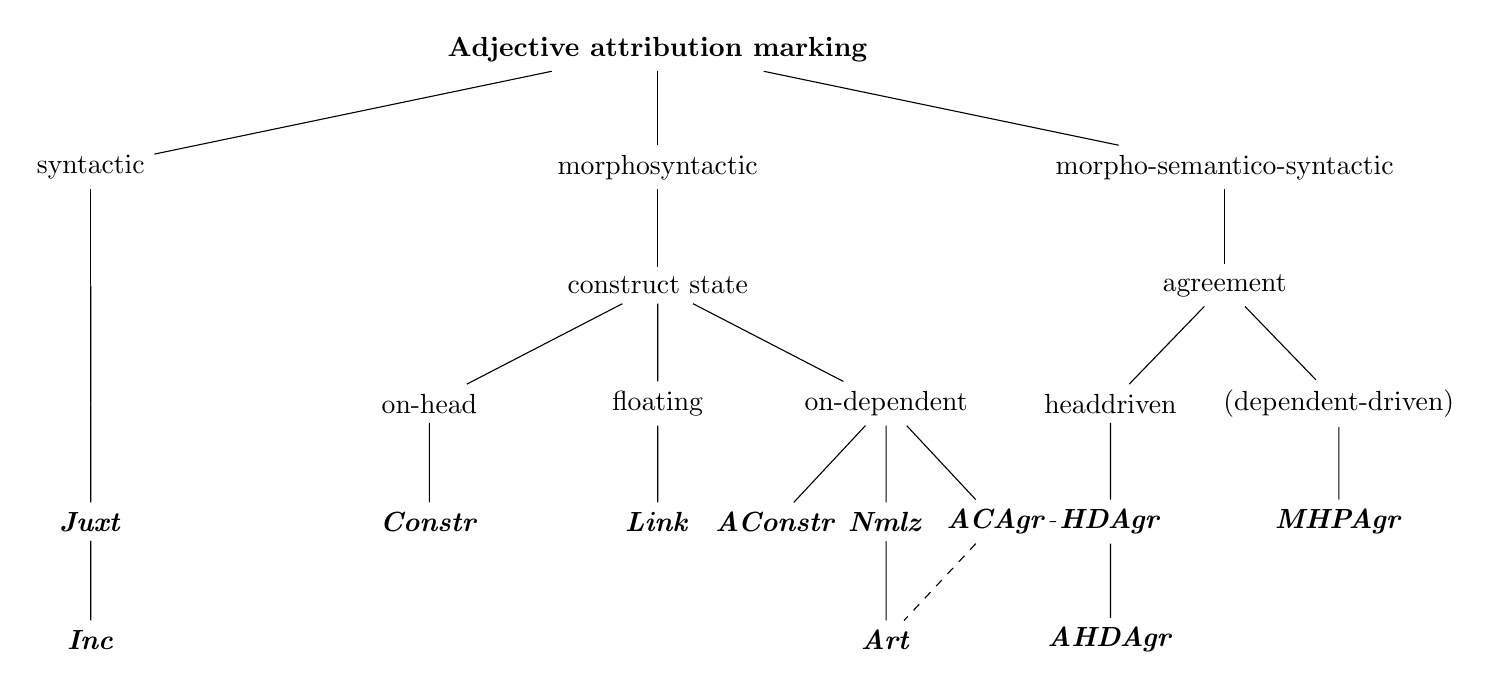
\begin{tikzpicture}
\tikzstyle{level 1}=[sibling distance=72mm]
\tikzstyle{level 3}=[sibling distance=29mm]
\tikzstyle{level 4}=[sibling distance=14mm]
\node {\textbf{Adjective attribution marking}}
child {node {syntactic}
	child {
		child {
			child {node {\textbf{\textit{Juxt}}}
				child {node {\textbf{\textit{Inc}}}
				}
			}
		}
	}
}
child {node {morphosyntactic}
	child {node {construct state}
		child {node {on-head}
			child{node {\textbf{\textit{Constr}}}
			}
		}
		child {node {floating}
			child{node {\textbf{\textit{Link}}}
			}
		}
		child {node {on-dependent}
			child{node {\textbf{\textit{AConstr}}}
			}
			child{node {\textbf{\textit{Nmlz}}}
				child{node (Art) {\textbf{\textit{Art}}}
				}
			}
			child{node (ACAgr) {\textbf{\textit{ACAgr}}}
			}
		}
	}
}
child {node {morpho-semantico-syntactic}
	child {node {agreement}
		child {node {head\hyp{}driven}
			child {node (HDAgr) {\textbf{\textit{HDAgr}}}
				child {node {\textbf{\textit{AHDAgr}}}
				}
			}
		}
		child {node {(dependent-driven)}
			child {node {\textbf{\textit{MHPAgr}}}
			}
		}
	}
};
\draw [dashed] (HDAgr) -- (ACAgr) -- (Art);
\end{tikzpicture}
\caption[Ontology of adjective attribution marking types]{Ontological tree of attested adjective attribution marking devices; type abbreviations are: ACAgr=Anti\hyp{}construct state agreement, AConstr=Anti\hyp{}construct state, AHDAgr=Appositional head\hyp{}driven agreement, Art=Attributive article, Constr=Construct state, HDAgr=Head\hyp{}driven agreement, Inc=Incorporation, Juxt=Juxtaposition, Link=Linker, MHPAgr=Modifier\hyp{}headed possessor agreement, Nmlz=Attributive nominalization} 
\label{tree ontology}
\end{sidewaysfigure}

\is{juxtaposition|)}
\is{incorporation|)}
\is{construct state|)}
\is{linker|)}
\is{anti\hyp{}construct state|)}
\is{attributive nominalization|)}
\is{attributive article|)}
\is{anti\hyp{}construct state agreement|)}
\is{head\hyp{}driven agreement|)}
\is{modifier\hyp{}headed possessor agreement|)}
